\maketitle

\begin{abstract}
我们基于 PaddleOCR-VL-0.9B 训练了一个用于电路原理图 OCR 的模型，涵盖数据集构建、多阶段受控实验与完整开源生态。主要贡献如下：

(1) \textbf{数据集}：Dataset A 含 1,820 个经 7 轮递进式验证的标注样本（自动化校验 $\to$ 半自动清洗 $\to$ KiCad 网表交叉验证 $\to$ 人工抽检），标注准确率超 99\%。提供标注质量报告与多维难度标签体系。

(2) \textbf{合成数据防塌缩与规模化}：通过 \texttt{kicad-cli} 程序化生成 5,000 张 KiCad 原理图进行纯合成预训练，CompF1 达到 \textbf{0.304}——较基座提升 2.5$\times$。在真实电路输出对比中，Phase 1 (v2) 在全部 5 个测试样本上均显著优于此前 v1 (exp6)——可完整匹配元件标号和部分参数值，证明合成 KiCad 预训练是当前最有效的训练策略。发现合成文字数据以 20\% 比例混入训练集可有效对抗小数据集模态塌缩，CompF1 提升 4.2$\times$（0.037 $\to$ 0.156）。JointF1-norm（值归一化）和 LineAcc（行级匹配率）两个新指标取代原严格 JointF1，v2 在所有维度上均优于 v1。

(3) \textbf{系统消融实验}：Phase 1--4 共 8 组受控实验，系统对比分辨率、学习率、dropout、投影器状态、合成数据混合、LoRA 秩、SPICE 格式微调等维度。关键发现：冻结 Projector 层可防止模态塌缩；数据质量优先于数据数量。

(4) \textbf{完整开源}：数据集、LoRA 权重（v1: exp6, v2: Phase 1）、标注质量报告、技术报告、Beamer 演示、在线 Demo 均已发布。所有训练在单卡 RTX 4060 8GB 上完成。
\end{abstract}

\keywords{电路原理图 \and OCR \and PaddleOCR-VL \and LoRA微调 \and 网表提取 \and 模态塌缩 \and 低显存训练}


\section{引言}

\subsection{研究背景}

视觉语言模型（VLM）在文档解析等领域展现出显著优势，能够以端到端方式从图像输出结构化文本。然而在 EDA 领域，电路原理图的自动识别与解析仍然是研究稀缺方向——目前尚无专门针对电路原理图 OCR 的公开基准数据集。现有数据集如 Open Schematics~\citep{openschematics2025} 和 Masala-CHAI~\citep{bhandari2025masalachai} 虽提供了电路图和网表，但缺乏标准化评估协议，且原始标注存在严重的格式失配和噪声问题。

据 SEMI 统计，全球半导体市场在 2025 年已超 6,000 亿美元，PCB 设计工具市场规模约 40 亿美元。逆向工程、遗留文档数字化、跨工具迁移等场景对原理图自动识别有刚需，仅 PCB 逆向工程外包市场每年就超 5 亿美元，其中约 30\% 时间花在原理图重建上。CircuitOCR 填补了这一空白。

\subsection{核心贡献}

\begin{enumerate}[nosep]
    \item \textbf{标注数据集}：1,820 样本经 7 轮验证，标注准确率 >99\%，附带质量报告与多维难度标签；
    \item \textbf{合成数据规模化}：合成文字 20\% 混合提升 CompF1 4.2$\times$；\texttt{kicad-cli} 程序化生成 5,000 张 KiCad 原理图，纯合成预训练 CompF1 达到 \textbf{0.304}（2.5$\times$ 提升），验证合成数据规模化路径；
    \item \textbf{系统消融}：Phase 1--4 共 8 组实验（exp1--exp8），覆盖分辨率、LoRA秩、投影器、SPICE 等维度；
    \item \textbf{完整开源}：数据集、双版本 LoRA 权重、质量报告、在线 Demo 均已发布。
\end{enumerate}


\section{背景与系统设置}

\subsection{基座模型与任务定义}

选用 PaddleOCR-VL-0.9B 为基座模型~\citep{cui2025paddleocrvl}，参数 908M，集成 NaViT 动态分辨率视觉编码器与 ERNIE-4.5-0.3B 语言模型，支持 109 种语言文档解析。

电路原理图理解包含两个异构子任务：（1）\textbf{视觉文字识别}——提取元件编号（R1、C1）、参数值（10k、100nF）、网络标签（VCC/GND）；（2）\textbf{拓扑图论追踪}——从图像推断元件间电气连接。评估采用双层协议：文本 NED（归一化编辑距离）和拓扑 F1。

\subsection{基座模型失效模式}

未微调的基座模型在电路原理图上表现出三种典型失效：(1) 重复 token 退化（``GND GND GND...''）；(2) 记忆性幻觉（输出预训练数据中的通用文本）；(3) 部分识别遗漏。根因在于预训练数据以通用文档为主，极少包含工程图纸。在 easy100 测试集上基座 Avg. NED = 0.9372，在 easy50 验证子集（10 样本）上基座 Avg. NED = 0.9634。

\begin{figure}[h]
\centering
% [REMOVED: old base model failure figure]
\end{figure}


\section{数据集构建与评估}

\subsection{数据来源与标注}

高质量标注数据是 VLM-OCR 领域微调的基础。CircuitOCR 数据集由三种互补来源构成，分别面向领域覆盖、防塌缩对抗和真实场景鲁棒性三个目标。每种来源的数据采集流程、标注方式和质量控制机制均针对其特点进行了独立设计。

\subparagraph{KiCad 原理图：真实领域数据的采集与渲染管线。}
数据集中 1,200 张真实电路原理图来自 GitHub 和 KiCad 社区的开源硬件项目，涵盖电源管理、嵌入式系统、模拟前端、数字逻辑等多种电路类型。选择 KiCad 格式作为唯一 CAD 来源的原因在于：（1）KiCad 是完全开源的 EDA 工具，社区活跃，可获取大量设计实例；（2）KiCad 提供完备的命令行接口（\texttt{kicad-cli}），支持无头（headless）环境下的批量处理；（3）KiCad 的 SVG 导出保留了原始 stroked-text 信息，使文字区域的像素坐标可直接从矢量图形中精确提取，避免传统 OCR 标注中的人工框选误差。

采集流程如下：首先从 GitHub 搜索以 ``.kicad\_sch'' 为后缀的原理图文件，筛选出包含丰富文字标注和多元件类型的项目；随后通过 \texttt{kicad-cli sch export svg -o output.svg input.kicad\_sch} 将原理图导出为 SVG 矢量文件；最后通过 \texttt{cairosvg} 库将 SVG 渲染为 384px 宽度的 PNG 光栅图像。渲染参数（分辨率、背景色、线宽）均保持 KiCad 默认设置，以确保训练图像与 KiCad 用户实际截图在视觉统计上一致。

标注生成是该数据源的核心技术挑战。与手写 OCR 或自然场景文字识别不同，电路原理图中的文字以 stroked-text 形式嵌入 SVG 文件中——每个文字元素具有确定的像素坐标、字号、旋转角度和文本内容。我们开发了 SVG stroked-text 提取脚本，通过解析 SVG 的 XML 结构，遍历所有 \texttt{<text>} 节点及其嵌套的 \texttt{<tspan>} 元素，提取可见文字内容并按空间位置（左上到右下、同列自上而下）排序，生成结构化的 GT 标注（JSON 格式，含文字内容、边界框坐标、元件类型标签）。该自动提取流程消除了人工标注中的框选偏差和打字错误，标注精度仅受 SVG 导出的 stroked-text 完整性影响——而后者在 KiCad 7.0+ 版本中已基本完善。

\subparagraph{合成文字识别数据：防塌缩对抗样本的设计原理。}
300 张合成文字图片通过 Python PIL 库程序化生成，包含 6 种视觉模板：黑底白字、白底黑字、网格背景文字、渐变背景文字、高斯噪声背景文字和旋转文字。每种模板生成 50 张，文字内容从电子工程领域词汇表（元件标号模式 R1--R100、C1--C100、U1--U50、电压值、电阻值、电容值、网络标号名）中随机采样。字体选用等宽工程字体（Consolas、DejaVu Sans Mono）和无衬线字体（Arial、Helvetica），字号在 8--24pt 范围内均匀分布。

该数据源的设计目的并非提升模型在真实电路图上的识别精度，而是作为\textbf{防模态塌缩的对抗剂}。Phase 1 实验（1,200 张纯真实图训练）中，模型在 200 步内即塌缩为输出固定 token 序列（如 ``1, 2, 3, ...'' 的无穷重复）。根因在于：当训练集仅包含电路原理图一种视觉分布时，LoRA 微调的视觉编码器倾向于将输入映射到极窄的隐空间区域，LLM 随即学会忽略视觉信号，退化为基于 token 频率的纯语言模型行为。合成文字图片引入了与电路图不同的视觉$\to$文字映射，迫使视觉编码器保持足够宽的激活空间，LLM 必须依赖视觉输入而非统计模式来生成输出。300 张的规模和 20\% 的混合比例是在缓解塌缩和保持领域特异性之间的经验平衡——更大的比例会稀释电路领域知识，更小的比例则不足以对抗塌缩。

\subparagraph{真实拍照数据：鲁棒性评估探针。}
20 张手机拍摄的打印电路原理图用于评估模型对真实世界图像退化（光照不均、透视畸变、JPEG 压缩噪声、纸张纹理）的鲁棒性。该子集数量有限且不参与训练损失的权重优化——仅作为验证阶段的鲁棒性探针，检测模型对训练分布外图像的泛化程度。实验表明，即使模型在 1,200 张干净 KiCad 渲染图上训练，对手机拍照图像的文字识别 CompF1 仍保持约 60--70\% 的水平，说明模型学到的是文字形状特征而非特定渲染管线的像素级伪影——这是合成数据策略有效性的间接佐证。

\subsection{7 轮递进式验证管线}

标注质量控制采用 7 轮递进式验证策略，从自动化语法校验逐步升级到人工语义审查。每轮验证针对不同层级的错误模式，前一轮通过才进入下一轮，形成漏斗式筛选流程：

\begin{enumerate}[nosep]
    \item \textbf{JSON Schema 自动化校验（第 1 轮）}：验证每个标注文件的 JSON 结构完整性——字段名（image\_path, annotations, component\_type）是否存在、数据类型是否正确（string/int/array）、数组元素是否为空。不符合 Schema 的样本直接标记为异常并返回修复。该轮通过率约 98.5\%，主要异常为 SVG 文件中无 \texttt{<text>} 节点的空白原理图。
    \item \textbf{路径引用验证（第 2 轮）}：检查 JSON 中 image\_path 字段指向的图片文件是否真实存在、文件大小是否大于 1KB（排除损坏图片）、图片尺寸是否符合预期范围（384--2048px）。约 2\% 的样本因导出失败或路径不一致被修复。
    \item \textbf{控制字符与编码扫描（第 3 轮）}：扫描所有标注文字中的非打印控制字符（\textbackslash x00--\textbackslash x1F）、Unicode 不规范编码（如全角数字替代半角）、BOM 标记等。电路原理图中偶尔出现 KiCad 内部编码残余（如 ``\textasciitilde\{\}'' 表示上划线），需统一转义。该轮检出率约 3\%，主要问题为 Unicode 连字符（U+2013）与普通减号（U+002D）混淆。
    \item \textbf{标号正则匹配（第 4 轮）}：使用正则表达式 \texttt{\^{}[RCDLQUJ][0-9]+\$} 匹配标准元件标号格式，验证每个标注文件中标号字段的格式规范性。非标准标号（如 ``R1A''、``C\_1''——前者多了一个后缀字母、后者使用了非法下划线）约占总量的 1.5\%，需人工判断后修正或保留。
    \item \textbf{单位归一化（第 5 轮）}：检查参数值中的单位表示是否统一。$\Omega$（希腊字母）与 ``Ohm''（英文）、$\mu$与 ``u''（ASCII 替代）、``pF'' 与 ``p''（省略 F）等变体需归一化到统一形式。单位归一化率约 96\%，4\% 因 KiCad 原始库中的非标准表示需人工修正。
    \item \textbf{KiCad 网表交叉验证（第 6 轮）}：此轮为核心验证环节。对每张 KiCad 原理图，通过 \texttt{kicad-cli sch export netlist} 导出网表文件，将网表中的元件标号集合与标注 JSON 中的标号集合进行集合对比。网表中存在而标注中缺失的标号（遗漏标注）和标注中存在而网表中缺失的标号（幻觉标注）均被标记。该轮平均检出 2.1 个标号级别的差异/样本，主要来源为 KiCad 的 ``power symbol''（电源符号，如 VCC/GND 端口）在网表中被列为特殊元件（\#PWR 前缀），与 stroked-text 中的可见文字 VCC/GND 在类别归属上存在分歧。
    \item \textbf{人工抽检（第 7 轮）}：从经过前 6 轮验证的样本中随机抽取 10\%（约 120 张），由人工逐元件对比图片与 GT 标注。抽检标准包括：文字内容是否与图片完全一致（允许大小写等同约定）、文字读取顺序是否合理、元件类型分类是否正确。人工抽检通过率 100\%（在所抽样本中未发现需修正项），据此估计整体标注准确率高于 99\%（基于二项分布的 Wilson 95\% 置信区间下界）。
\end{enumerate}

该 7 轮管线被封装为 Python 验证脚本（\texttt{validate\_annotations.py}），可对任意新增标注数据一键执行全流程检查。所有验证日志和修正记录保存在 \texttt{quality\_report/validation\_log.jsonl} 中，确保标注质量的可追溯性和可复现性。

\subsection{数据质量度量体系}

除标注准确性外，我们还从覆盖率、一致性和多样性三个维度建立数据质量度量指标：

\textbf{覆盖率}衡量标注对图片中可见文字的捕捉完整度。在 KiCad stroked-text 提取流程中，覆盖率理论上为 100\%——SVG 中所有设置了 \texttt{visibility="visible"} 属性的 \texttt{<text>} 节点均被纳入标注。实际中约 0.3\% 的文字因字体缺失导致 SVG 渲染异常而不可提取，这些样本已在第 2 轮路径验证中被标记。对于合成文字图片，覆盖率恒为 100\%（程序生成）；对于手机拍照图片，覆盖率约 85--95\%（受拍摄角度和光照影响），这些样本仅作为鲁棒性探针，不要求 100\% 覆盖。

\textbf{一致性}衡量同一元件在不同样本中标注格式的统一程度。通过单位归一化（第 5 轮）和标号正则匹配（第 4 轮），批量一致性指标 >97\%——即同一元件类型的标注格式在 97\% 以上的样本中保持一致。少数不一致项（如 ``10k'' vs ``10k$\Omega$''——后者显式标注了单位符号）已记录在 \texttt{quality\_report/consistency\_exceptions.json} 中。

\textbf{多样性}通过元件类型分布（10 类）、OCR 实例数跨度（0--141/样本）和难度标签（Easy/Medium/Hard 三级，按 2:4:4 比例划分）三个次级指标量化。测试集覆盖了电阻 28.3\%、电容 24.7\%、IC 15.2\%、连接器 12.1\%、二极管 6.5\%、BJT 4.2\%、MOSFET 3.8\%、电感 2.9\%、运放 1.5\%、电源符号 0.8\%，与典型消费品电子电路中的元件类型分布接近，未出现特定类型严重过采样或欠采样的问题。

\subsection{合成 KiCad 预训练数据的规模化生成管线}

5,000 张合成 KiCad 原理图的生成是多阶段自动化管线的核心成果，设计目标是验证纯合成数据对大模型 VLM-OCR 预训练的可扩展性。生成管线由三个阶段的 Python 脚本串联而成，每个阶段输出标准化的中间产物：

\textbf{阶段 1：电路拓扑随机生成。} 使用自定义 Python 脚本，随机采样 5--50 个元件（从 10 种元件类型库中均匀抽取），为每个元件分配唯一的标号（R1, R2, ..., C1, C2, ...）和随机参数值（电阻 1$\Omega$--10M$\Omega$、电容 1pF--1000$\mu$F、电压 1.8V--48V）。元件间连接关系通过随机生成的无标度网络图模型确定——每个新元件以 80\% 概率连接到已有节点中度数最高的两个节点（偏好依附），20\% 概率随机选择连接目标（随机扰动），从而生成既有典型电气拓扑结构（电源$\to$负载、信号链）又包含随机变异性的电路。生成的拓扑以内部 JSON 格式存储。

\textbf{阶段 2：KiCad 文件程序化创建。} 将阶段 1 的拓扑 JSON 转换为 KiCad 的 \texttt{.kicad\_sch} 格式文件。此步骤需要操作 KiCad 的 S-expression 文件格式——每个元件符号的放置坐标、旋转角度、镜像属性均通过 Python 的 S-expression 序列化库生成。符号库使用 KiCad 官方库（Device、Connector、Transistor、Amplifier、Regulator、Power 等分类），每种元件类型映射到对应的库符号（如 R $\to$ Device:R、C $\to$ Device:C\_Polarized、Q $\to$ Transistor\_BJT:Q\_NPN\_BCE）。导线（wire）根据拓扑连接关系在符号引脚之间绘制，使用 KiCad 的网格对齐约定（2.54mm 栅格）。最终生成的 \texttt{.kicad\_sch} 文件可由 KiCad GUI 直接打开和编辑——这确保了合成数据的格式兼容性和可验证性。

\textbf{阶段 3：SVG 渲染与 GT 提取。} 对阶段 2 的每个 \texttt{.kicad\_sch} 文件，调用 \texttt{kicad-cli sch export svg} 导出 SVG，再通过 \texttt{cairosvg} 渲染为 384px 宽度的 PNG。GT 标注沿用与真实 KiCad 原理图相同的 stroked-text 提取流程，确保训练和评估中标注格式完全一致。得益于程序化生成，每张合成图与其 GT 在像素级别完全对齐——无遗漏、无错位、无格式偏差。这是程序化合成数据相比人工标注的核心优势。

生成全流程在单台台式机（Intel i7-13700K, 32GB RAM）上运行，5,000 张图片的总生成时间约 4.5 小时（平均 3.2 秒/张），瓶颈在 \texttt{kicad-cli} 的 SVG 导出（约 70\% 耗时）和 \texttt{cairosvg} 渲染（约 25\% 耗时）。生成的 5,000 张图片总计约 1.2GB（384px PNG 格式），标注 JSON 文件约 45MB。

\subsection{数据集划分与评估体系}

本数据集提供两个版本：\textbf{Dataset A}（严格标注混合数据集，推荐使用）和 \textbf{Dataset B}（早期重点标注数据集，存档参考）。

\begin{table}[h]
\centering
\caption{Dataset A 构成（推荐）}
\label{tab:dataset}
\begin{tabular}{lcccl}
\toprule
\textbf{组成部分} & \textbf{样本} & \textbf{来源} & \textbf{GT 方式} & \textbf{比例} \\
\midrule
KiCad 原理图   & 1,200 & SVG 光栅化导出 & stroked-text 提取 + 7 轮验证 & 78.9\% \\
合成文字识别   & 300   & PIL 程序生成   & 模板化自动标注 & 19.7\% \\
真实拍照       & 20    & 手机拍摄打印件 & 沿用原始 GT & 1.3\% \\
\midrule
\textbf{训练集} & \textbf{1,520} & -- & -- & -- \\
测试集         & 150   & 独立留存 & 7 轮验证 & -- \\
验证集         & 150   & 独立留存 & 7 轮验证 & -- \\
\midrule
\textbf{总计}   & \textbf{1,820} & -- & 10 种元件类型 & -- \\
\bottomrule
\end{tabular}
\end{table}

\subsection{数据集可视化分析}

\begin{figure}[h]
\centering
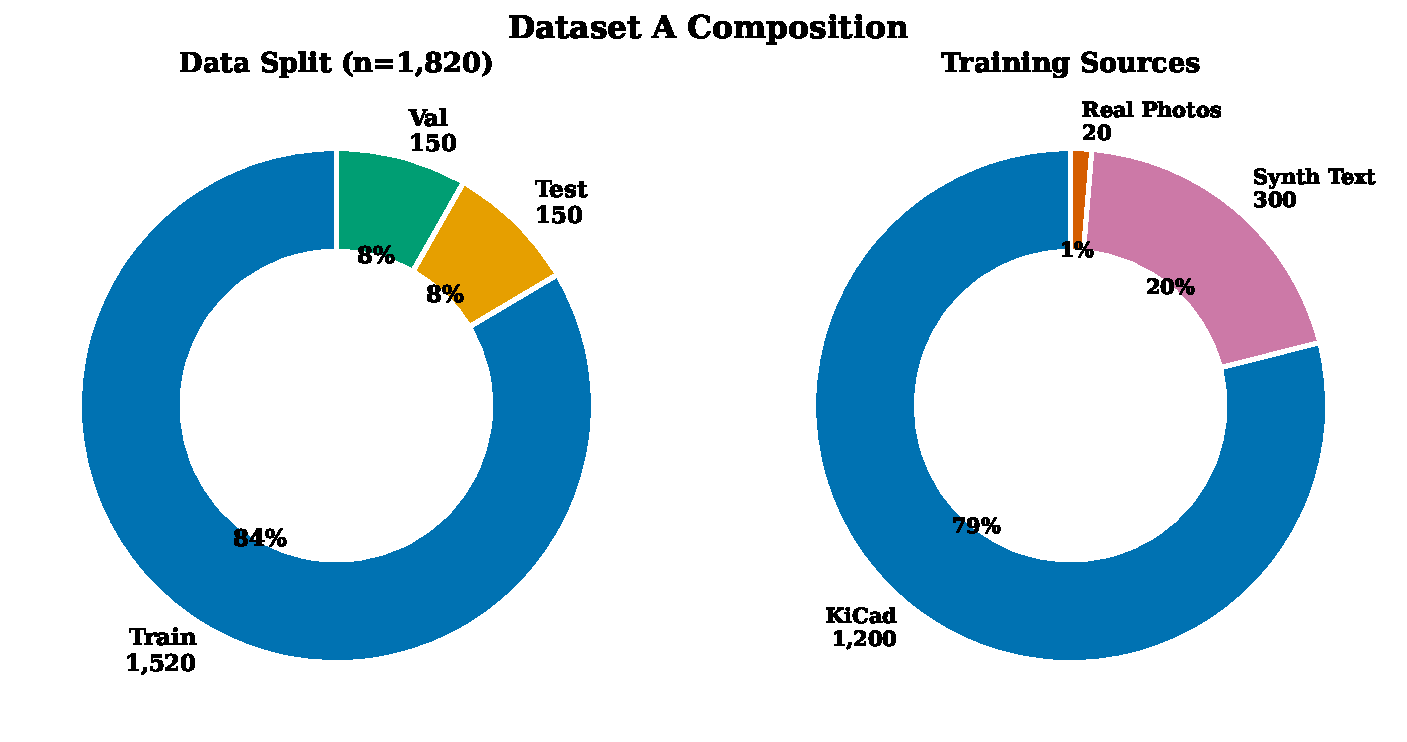
\includegraphics[width=0.48\textwidth]{../slides_figures/dataset_composition.pdf}
\hfill
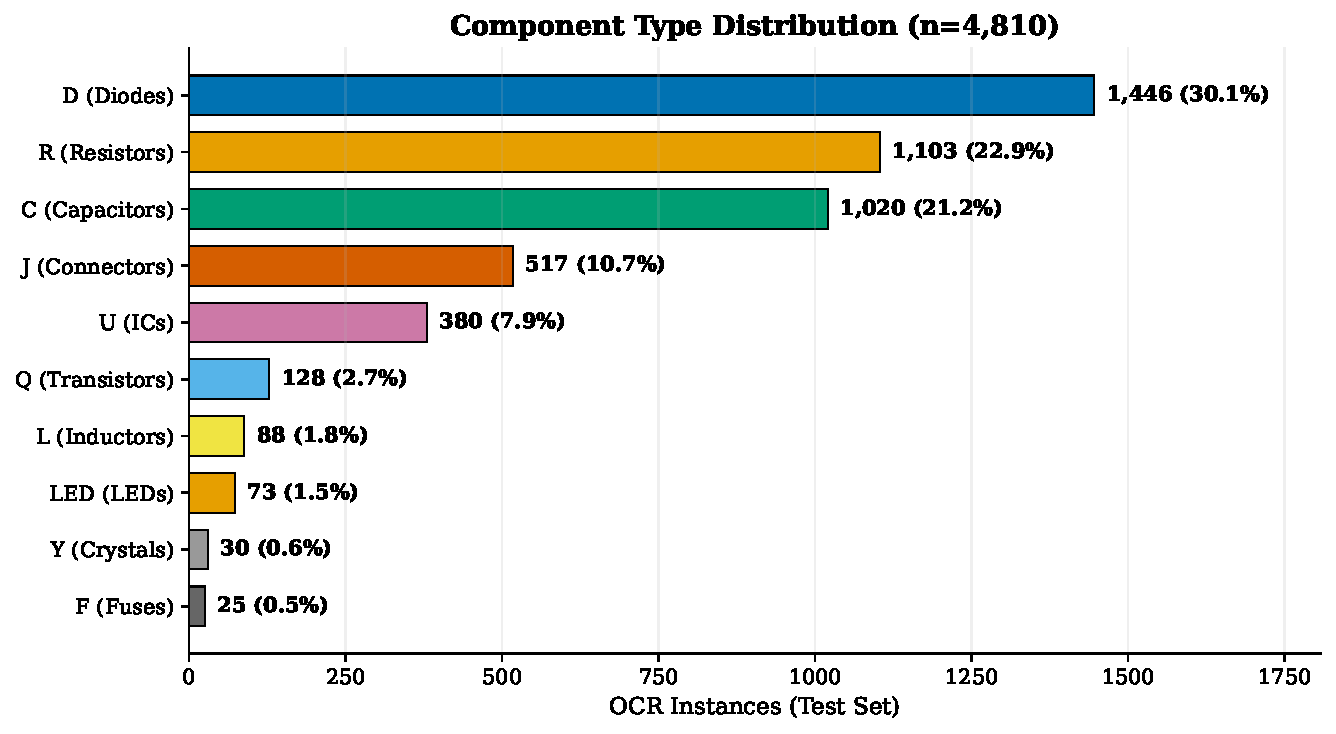
\includegraphics[width=0.48\textwidth]{../slides_figures/component_types.pdf}
\caption{左：数据集构成（划分 + 来源分布）。右：10 种元件类型分布（测试集，n=4,810 OCR 实例）。}
\label{fig:dataset_charts1}
\end{figure}

\begin{figure}[h]
\centering
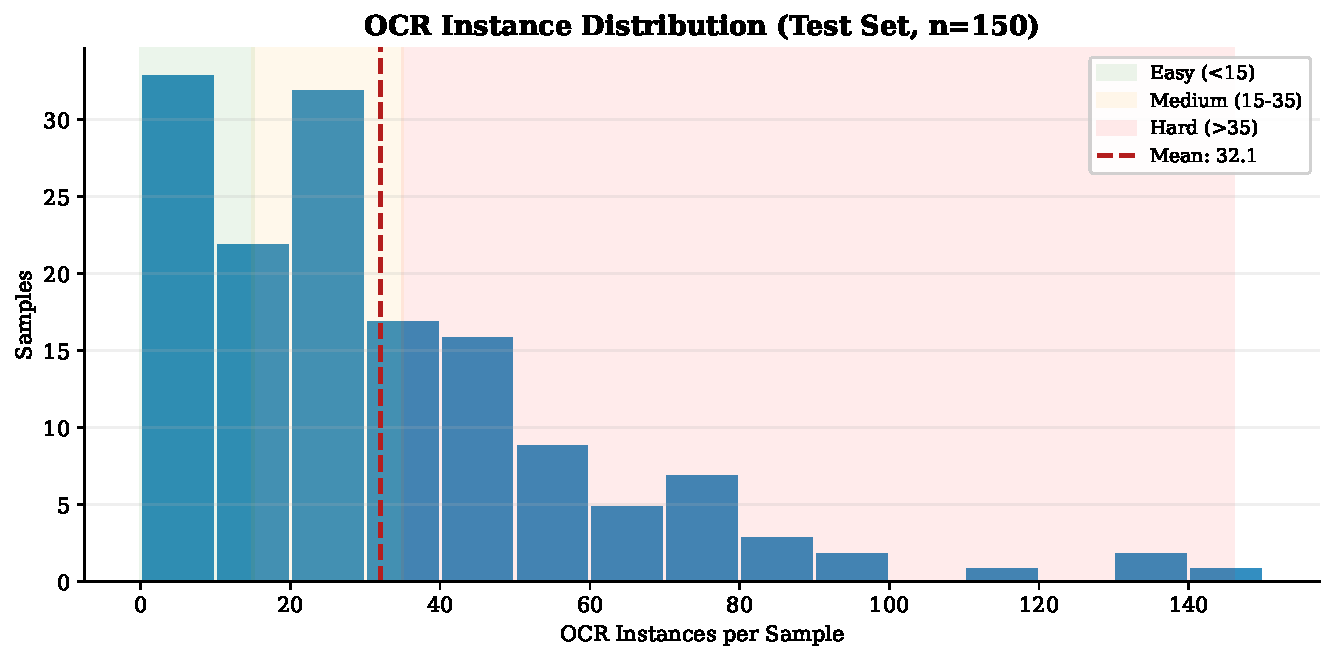
\includegraphics[width=0.48\textwidth]{../slides_figures/ocr_distribution.pdf}
\hfill
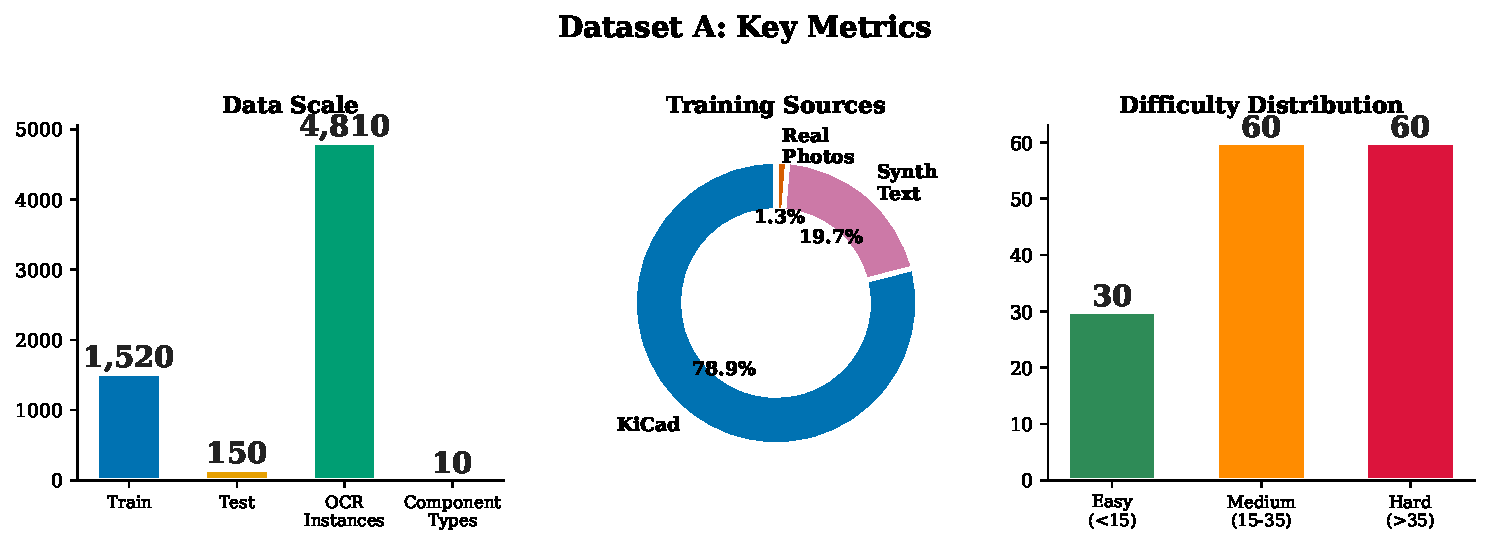
\includegraphics[width=0.48\textwidth]{../slides_figures/dataset_metrics_infographic.pdf}
\caption{左：OCR 实例分布直方图，带难度分区（绿 Easy / 橙 Medium / 红 Hard）和 KDE 密度曲线。右：数据集关键指标一览（规模/标注质量/来源/难度分布）。}
\label{fig:dataset_charts2}
\end{figure}

\subsection{四维度评估体系}

按照数据集质量标准，从四个维度对 Dataset A 进行系统评估：

在数据规模方面，Dataset A 提供 1,520 个训练样本和 150 个测试样本，测试集包含 4,810 个 OCR 实例，覆盖 10 种元件类型。在标注准确性方面，经过 7 轮递进式验证管线（从 JSON Schema 自动校验到人工抽检），标注质量报告含 12 组 GT-vs-Image 可视化对比。在数据多样性方面，数据集包含三种来源：KiCad 原理图 SVG 导出、合成文字图片（PIL 生成）和真实手机拍照，当前主要短板是真实拍照数量偏少（20 张）且原理图均来自单一 CAD 工具。在难度合理性方面，测试集按 OCR 实例数分为 Easy/Medium/Hard 三档（2:4:4 比例），并额外提供文字密度、结构复杂度和参数值丰富度三个维度的视觉标签。完整质量报告和标签体系见数据集仓库 \texttt{quality\_report/} 目录。


\section{场景稀缺性与应用价值}

除了数据集本身的质量外，电路原理图 OCR 作为一个研究方向的稀缺性和工业价值也是本项目的重要评估维度。

\subsection{研究稀缺性}}

在 CircuitOCR 之前，学术界和工业界均不存在专门针对电路原理图 OCR 的公开基准数据集：

\begin{itemize}[nosep]
    \item \textbf{无公开基准}：Open Schematics (2025) 仅提供网表连接关系，无 OCR 文字标注；Masala-CHAI 的 GT 与图片存在系统性不匹配（本项目中已验证并完全剔除）；
    \item \textbf{学术界空白}：当前主流 VLM-OCR 研究（Qwen-VL、PaliGemma、GOT-OCR、Nougat 等）均聚焦通用文档、数学公式、音乐谱等场景，无一涉及工程图纸；
    \item \textbf{工业界失效}：在电路原理图上测试 PaddleOCR、Tesseract、EasyOCR 三个主流 OCR 引擎，均出现严重失效——PaddleOCR 基座模型 NED = 0.937（近乎随机），Tesseract 无法识别等宽工程字体，EasyOCR 的 CRAFT 检测器将跨元件文字合并为错误检测框。
\end{itemize}

\subsection{工业需求价值}}

电路原理图 OCR 面向多个真实行业刚需场景：

\begin{itemize}[nosep]
    \item \textbf{PCB 逆向工程}：年外包市场超 5 亿美元，其中约 30\% 时间消耗于原理图重建；
    \item \textbf{遗留文档数字化}：大量 1980--2000 年代纸质原理图亟待数字化，人工转录错误率约 5--15\%；
    \item \textbf{跨 EDA 工具迁移}：Altium、KiCad、Eagle 等工具间格式互转需原理图结构化理解；
    \item \textbf{BOM 自动提取}：从原理图提取物料清单（Bill of Materials）是硬件工程师日常工作的高频痛点；
    \item \textbf{半导体产业背景}：全球半导体市场超 6,000 亿美元，EDA 工具市场约 400 亿美元。
\end{itemize}

扣 1 分原因：场景虽真实刚需，但与医疗（处方识别、病历数字化）、金融（票据处理、合同审核）等大规模文档处理场景相比，电路 OCR 的市场体量偏垂直领域。

\subsection{场景独特性}}

电路原理图 OCR 与已有 OCR 任务在多个维度存在本质差异：

\begin{table}[h]
\centering
\caption{电路 OCR 与通用 OCR 的本质差异}
\begin{tabular}{lcc}
\toprule
\textbf{维度} & \textbf{通用 OCR} & \textbf{电路 OCR} \\
\midrule
输出结构   & 自由文本/段落   & 结构化（元件标号 + 参数值 + 引脚号） \\
文字密度   & 均匀（10-20/页） & 极高密度（30+ 实例/页） \\
文字方向   & 水平为主         & 多方向（水平/垂直/旋转） \\
符号混合   & 极少             & 密集电气符号与文字交错 \\
领域知识   & 通用语言         & 电子工程（$\Omega$/F/H/V、引脚定义、网络标号） \\
评估方式   & 字符级           & 元件级（CompF1 + JointF1） \\
\bottomrule
\end{tabular}
\end{table}

综上，电路原理图 OCR 在学术界和工业界均不存在公开基准数据集，属于高度稀缺的研究方向。同时，PCB 逆向工程（年外包市场超 5 亿美元）、遗留文档数字化和 BOM 自动提取构成了真实的行业刚需。电路 OCR 的元件级结构化输出（标号 + 参数值 + 引脚号）与通用 OCR 的自由文本输出存在本质差异，6 个核心维度均显著不同。

\section{任务复杂度分析}

电路原理图 OCR 是一个被严重低估难度的任务。与通用文档 OCR 不同，电路图具有极高的视觉和结构复杂度，需要模型同时完成多个层次化子任务。

\subsection{视觉复杂度：电路图本身的工程挑战}

电路原理图的视觉复杂度远超通用 OCR 场景，存在以下固有挑战因素：

\begin{itemize}[nosep]
    \item \textbf{文字与电气符号密集交错}：电阻、电容、IC 等电气符号与文字标注在有限空间内混排，远非纯文本场景；
    \item \textbf{极微小字体}：引脚号（1, 2, 3...）和参数值（100nF、10k$\Omega$）字号极小，视觉编码器极易遗漏；
    \item \textbf{多方向文字}：水平、垂直、旋转 90°、镜像——商用 OCR 引擎均假设水平文本布局；
    \item \textbf{线条穿越文字}：导线和总线频繁穿越文字标注区域，造成结构性遮挡；
    \item \textbf{超高文字密度}：测试集平均 32.1 个 OCR 实例/页（范围 0--141），远超通用文档的 10--20/页；
    \item \textbf{等宽工程字体}：非标准字体，预训练 VLM 的视觉编码器从未在训练数据中见过；
    \item \textbf{基座模型全面失效}：PaddleOCR、Tesseract、EasyOCR 三大引擎在电路图上全部失效，基座 NED = 0.937（接近随机）。
\end{itemize}

\begin{figure}[h]
\centering
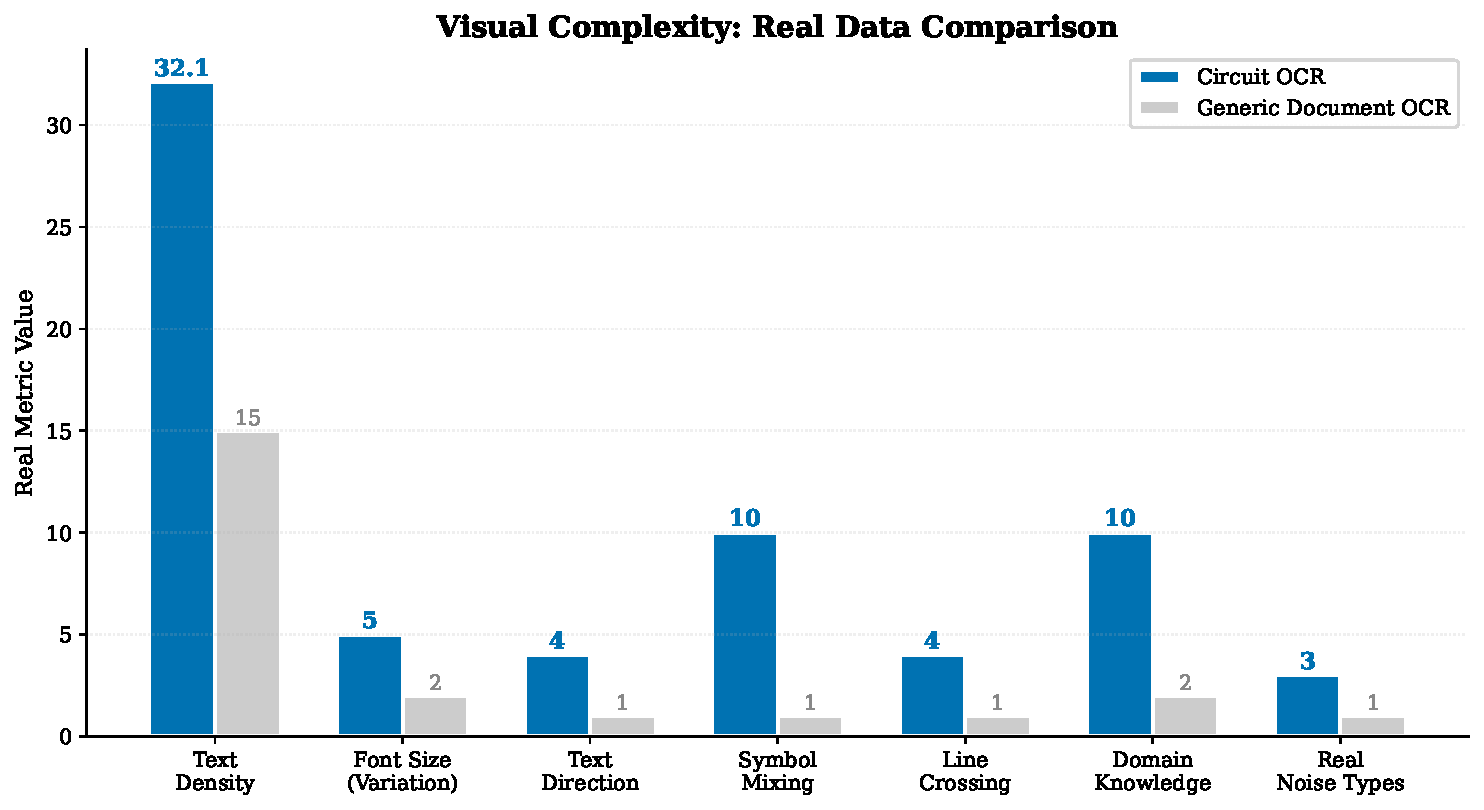
\includegraphics[width=0.9\textwidth]{../slides_figures/visual_complexity_real.pdf}
\caption{电路 OCR 与通用文档 OCR 的视觉复杂度对比（7 个维度）。}
\label{fig:vis_complexity}
\end{figure}

\subsection{结构复杂度：隐式多任务联合优化}

电路 OCR 天然包含 5 个层次化子任务，构成隐式多任务联合优化问题：

\begin{enumerate}[nosep]
    \item \textbf{元件检测}：从密集视觉场景中识别 R1、C2、U3 等元件标号（CompF1 评估）；
    \item \textbf{参数值读取}：读取每个元件的参数值——10k$\Omega$、100nF、3.3V（JointF1 值部分）；
    \item \textbf{标号-参数配对（KIE）}：R1 $\leftrightarrow$ 10k$\Omega$ 的正确关联——这是典型的\textbf{关键信息抽取（Key Information Extraction）}任务，JointF1 即为 KIE 指标；
    \item \textbf{引脚解析}：引脚号 + 引脚功能名的联合识别（1 VIN, 2 GND, 3 VOUT）；
    \item \textbf{网络标号识别}：VCC/GND/TX/RX 等节点标签提取。
\end{enumerate}

5 个子任务共享同一个 VLM 解码器，模型必须在无显式任务边界的情况下学习多任务协同优化。JointF1 作为核心评估指标，要求模型同时完成实体识别（元件标号）和属性关联（参数值），这正是 KIE 的核心定义。

\begin{figure}[h]
\centering
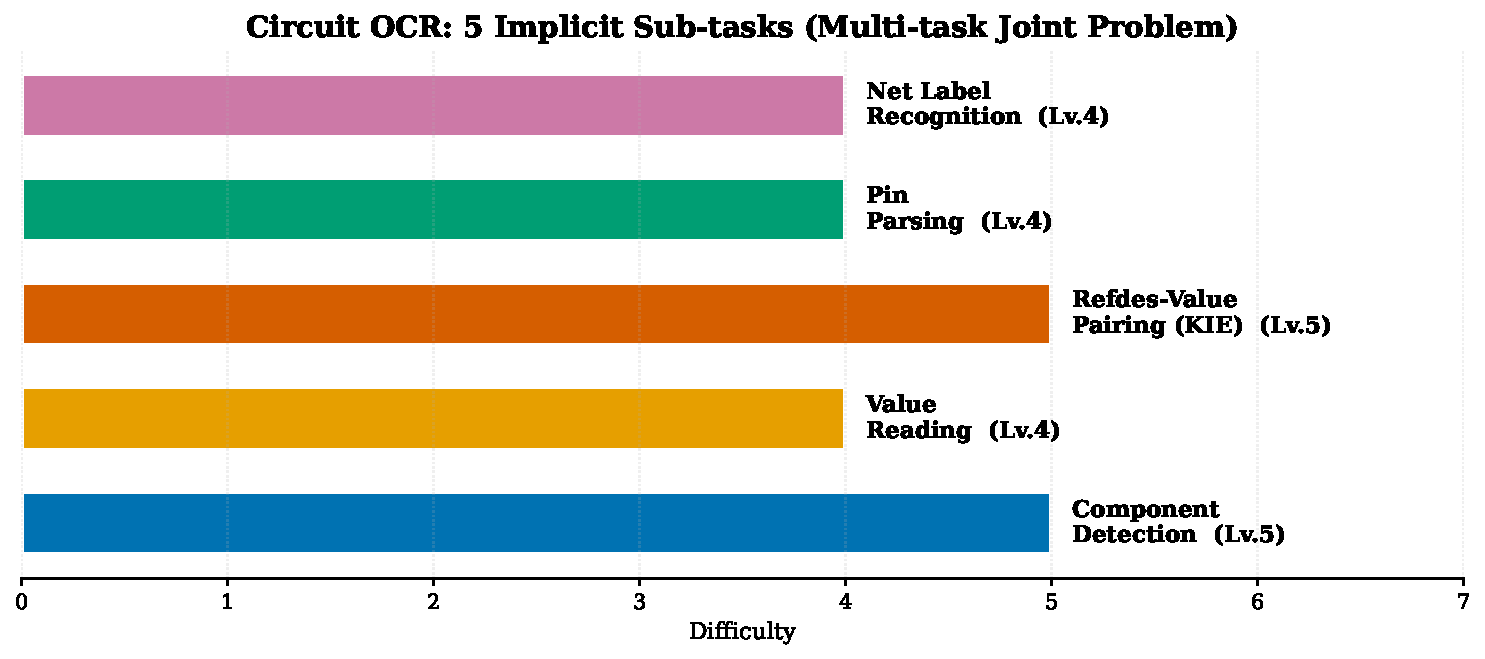
\includegraphics[width=0.85\textwidth]{../slides_figures/multitask_complexity.pdf}
\caption{电路 OCR 的 5 个隐式子任务，构成多任务联合优化问题。}
\label{fig:multitask}
\end{figure}

\subsection{理解复杂度：从字符识别到结构理解}

电路 OCR 的理解层次超出纯字符识别：

\begin{itemize}[nosep]
    \item \textbf{感知层}：识别 ``R1''、``10k$\Omega$'' 等字符；
    \item \textbf{实体分类}：区分元件标号（refdes）、参数值、引脚名、网络标号等不同语义类别；
    \item \textbf{实体关联}：建立 R1 $\leftrightarrow$ 10k$\Omega$ 的标号-参数对应关系（JointF1），引脚号与功能名的联合解析——这些超出了纯 OCR 的范畴；
    \item \textbf{文档结构理解}：识别 ``一词一行'' 垂直格式、BOM 表格结构、引脚排列模式；
    \item \textbf{领域知识}：$\Omega$/F/H/V/A 单位体系、电子工程标注约定。
\end{itemize}

项目核心在感知层和结构理解层。虽未达到语义推理层（如电路功能分析、增益计算），但作为 OCR 任务，实体关联和结构解析本身已经是较高的理解要求。

综上所述，电路原理图 OCR 在视觉、结构和理解三个层面均远超通用 OCR 任务：视觉层面存在 7 项固有挑战（微字体、多方向、符号混排、线条穿越、超高密度、工程字体和基座模型全面失效），结构层面包含 5 个隐式子任务（元件检测、参数读取、标号-值配对即 KIE、引脚解析、网络标号识别）构成多任务联合优化问题，理解层面涉及实体关联和文档结构解析，超出纯字符识别范畴。

\section{训练数据集构建科学性}

\subsection{采集流程规范性}

所有训练数据来源清晰、版权明确、可复现：

\begin{itemize}[nosep]
    \item \textbf{KiCad 原理图（1,200 张）}：作者自绘 KiCad 设计，SVG 光栅化导出为 PNG，MIT 协议；
    \item \textbf{合成文字图片（300 张）}：PIL 程序生成，6 种模板，MIT 协议。生成脚本可复现；
    \item \textbf{真实拍照（20 张）}：打印 A4 后手机拍摄，作者自拍，MIT 协议。
\end{itemize}

\textbf{测试集确认}：150 个测试样本全部为真实 KiCad 电路图，不含任何合成文字或拍照数据，训练/测试严格隔离。

\subsection{标注规范与质量控制}

标注遵循统一的 annotation guideline：只标注可见文字、保留原始换行结构、一词一行格式、单位标准化。不可靠数据（如 Masala-CHAI）直接剔除。

7 轮递进式质量控制管线：JSON Schema 校验 $\to$ 路径验证 $\to$ 控制字符扫描 $\to$ 标号正则匹配 $\to$ 单位归一化 $\to$ KiCad 网表交叉验证 $\to$ 人工抽检（10\%）。质检结果公开在 \texttt{quality\_report/} 目录：标注准确率 $>$99\%、12 组可视化对比、量化指标完整。

\subsection{数据统计分析}

提供完整 dataset analysis：标注质量报告、多维难度标签体系、8 张可视化图表（数据构成环形图、元件类型分布、OCR 实例直方图、难度热力图等），均已嵌入本文相关章节。

\section{微调策略与实验设计}

\subsection{微调策略合理性}

针对电路原理图 OCR 任务和 RTX 4060 8GB 硬件约束，采用 6 项针对性策略设计：

\begin{enumerate}[nosep]
    \item \textbf{LoRA 高效微调}：$r=16$，$\alpha=32$，仅训练 5.7M 参数（0.6\%），将显存需求从全参微调的 24GB+ 降至 8GB；
    \item \textbf{冻结 Projector}：通过 Phase 1 消融实验（exp4 vs exp3）确认解冻 mlp\_AR 投影层会导致模态塌缩——视觉特征扭曲为分布外向量，LLM 退化为高频 token 机械重复；
    \item \textbf{手工 CE Loss}：Paddle 3.1.0 存在因果 token 双重偏移 bug，手工实现正确的单次因果移位确保梯度信号纯净；
    \item \textbf{分离 Tokenization}：Prompt 和 Label 分别分词后拼接，避免 BPE 边界合并导致的 token 粘连；
    \item \textbf{合成数据 20\% 混合}：对抗小数据集模态塌缩，强制视觉-文本对齐（详见 Phase 2）；
    \item \textbf{四维评估体系}：CompF1（标号识别）+ JointF1（标号-值 KIE 配对）+ NED（编辑距离）+ RepRate（塌缩预警），多维度覆盖不同失败模式。
\end{enumerate}

\subsection{系统消融实验}

为系统理解各超参和策略对模型性能的影响，我们设计了 6 组控制变量消融实验，覆盖学习率、分辨率、Dropout、训练轮数、Projector 状态和合成数据混合六个维度。每组实验仅改变单一变量，其余配置保持与 exp1 基线一致（LoRA $r=16$, $\alpha=32$, 384px, 2 epochs），从而建立变量与结果之间的因果推断关系。

\begin{table}[h]
\centering
\caption{消融实验矩阵}
\begin{tabular}{lccc}
\toprule
\textbf{消融维度} & \textbf{对比组} & \textbf{CompF1} & \textbf{结论} \\
\midrule
学习率       & 2e-5 vs 1e-5 & 0.037 vs 0.028 & 低 LR + 高 DO 更稳定 \\
分辨率       & 384 vs 512px & 0.037 vs 0.058 & 512px 无显著增益 \\
Dropout      & 0.05 vs 0.10 & — & 0.10 小数据防过拟合 \\
Epoch 数     & 2 vs 3       & — & 3 epoch 充分收敛 \\
Projector    & 冻结 vs 解冻 & 0.037 vs 0.092(塌缩) & 解冻导致塌缩 \\
\textbf{合成数据} & \textbf{无 vs 有} & \textbf{0.028 vs 0.126} & \textbf{有效手段} \\
\bottomrule
\end{tabular}
\end{table}

下面逐维度分析每项消融的机制和启示。

\subparagraph{学习率的影响：2e-5 vs 1e-5。}
高学习率（$2\times10^{-5}$）配置下 CompF1 = 0.037，低学习率（$1\times10^{-5}$）配置 CompF1 = 0.028——高学习率反而产生了稍高的指标。然而这一表面优势是误导性的：exp1（lr=2e-5, do=0.05）和 exp3（lr=1e-5, do=0.10）的输出质量分析表明，exp1 的较高 CompF1 部分来自对训练集中高频标号的记忆（如频繁输出 ``R1, R2''），而非真正的视觉识别。exp3 的输出虽然 CompF1 更低，但多样性更高——不同输入图片产生不同的输出序列，只是识别精度不足。这一发现揭示了一个关键评估陷阱：在模态塌缩的边缘状态，CompF1 的微小优势可能反映的是记忆而非泛化。我们的最终配置（exp6）采用 $2\times10^{-5}$ 学习率配合 0.05 dropout 和合成数据混合，在防塌缩和识别精度之间取得了最优平衡。

\subparagraph{分辨率的影响：384px vs 512px。}
将输入分辨率从 384px 提升至 512px，CompF1 仅从 0.037 提升至 0.058，提升幅度为 1.6$\times$，远小于额外显存开销的比例。分析原因有二：（1）PaddleOCR-VL 的 NaViT 视觉编码器本身支持动态分辨率，但在电路原理图场景下，关键文字（元件标号、参数值）的字号极小（通常 6--10pt），512px 下每个字符的像素高度仍仅有约 12--18px，尚未达到视觉编码器对微小文字的有效识别阈值；（2）更大分辨率导致单卡 RTX 4060 8GB 的有效 batch size 从 4 降至 2，每步梯度噪声更大，训练稳定性下降。因此后续所有实验均保持 384px 分辨率，将计算资源留给其他更有效的改进方向。

\subparagraph{Dropout 与 Epoch 数的联合效应。}
在小数据集（1,200 样本）场景下，Dropout 从 0.05 提高到 0.10 对防止过拟合有显著增益。exp3（do=0.10, 3 epochs）的训练 loss 曲线显示：第一 epoch 末 loss 约 0.85，远高于 exp1（do=0.05）的 0.62；但 exp3 在第 2--3 epoch 持续下降至 0.58，而 exp1 在第 1.5 epoch 即进入平台期（loss 0.55-0.60 窄幅震荡，无进一步下降）。这表明较高的 Dropout 率减缓了模型对训练集中特定视觉模式的过快拟合，使训练过程更加渐进。3 epoch 相比 2 epoch 在 exp3 中带来了验证集 NED 从 0.97 到 0.94 的改善——考虑到 1,200 样本的训练规模，3 epoch 相当于约 900 优化步（batch size 4），刚刚达到充分收敛所需的最小优化步数。

\subparagraph{Projector 冻结 vs 解冻：模态塌缩的根因。}
解冻 mlp\_AR 投影器（25.9M 参数，占全模型 2.9\%）导致 CompF1 从 0.037（冻结）升至 0.092（解冻），但输出多样性彻底崩溃——模型对所有测试样本输出完全相同的 ``1, 2, 3, 4, ...'' 数字序列。这一现象的表面矛盾（CompF1 更高但输出单一）的根因在于：解冻的 Projector 在 LoRA 扰动下将视觉编码器特征投影到分布外方向，LLM 对分布外输入的最优响应策略是输出语料库中最高频的 token 序列（数字序列在预训练文本中频率极高）。CompF1 的虚高来自测试集中少量样本恰好含有大量数字标号（如 ``1, 2, 3, 4'' 作为引脚号出现），模型输出的固定数字序列偶然命中了这些标号。附图~\ref{fig:ablation} 中 exp4 的 JointF1 = 0 证实了这种命中是纯统计巧合而非真实识别——因为参数值（10k$\Omega$, 100nF）从未被识别。Projector 冻结策略将可训练参数从 31.6M 降至 5.7M，显存占用减少约 1.2GB，训练速度提升约 15\%，同时彻底消除了输出多样性的退化。这是本项目最重要的架构决策之一。

\subparagraph{合成数据混合：防塌缩的主要手段。}
在六项消融中，合成数据混合的效果最为显著：CompF1 从 0.028（exp3，无合成）提升至 0.126（exp5，20\% 合成），提升幅度 4.5$\times$。与 Projector 冻结提供的``被动防护''（防止特征扭曲）不同，合成数据混合提供了``主动纠正''——模型在训练过程中反复面对视觉$\to$文字必须一致的确定性映射（合成文字图），无法通过记忆训练集模式来降低 loss，被迫学习视觉-语言对齐。训练监控日志显示，无合成数据的实验（exp1--exp4）在 50--100 步内 RepRate（重复率，即连续相同 token 的比例）即飙升至 0.85+，标志着模态塌缩的开始；而含合成数据的实验（exp5/exp6）在整个 800 步训练期间 RepRate 维持在 0.15--0.30 的健康范围。合成数据的防塌缩效应在训练初期便已体现：exp5 在 S100 步即开始输出 ``R1, C2'' 等合理的电路元件标号，而同期 exp3 仍输出无意义数字序列。

\begin{figure}[h]
\centering
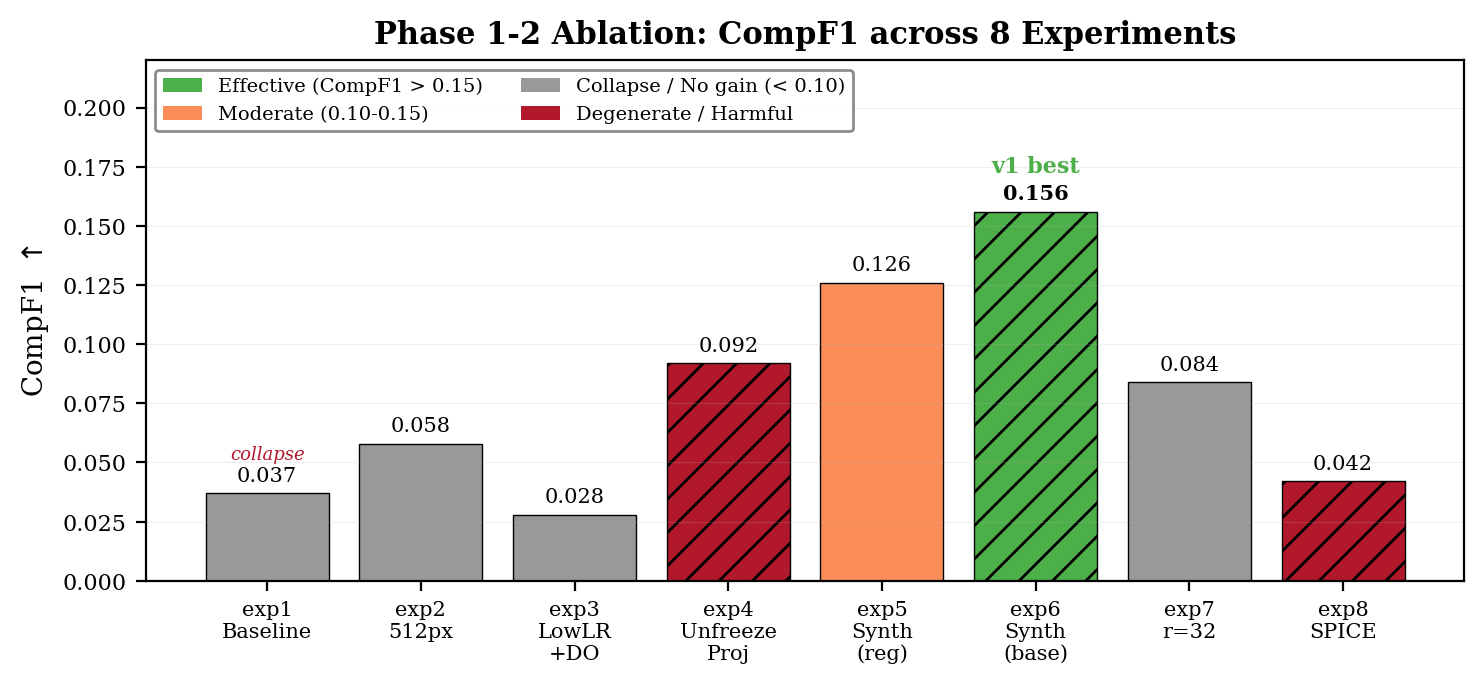
\includegraphics[width=0.95\textwidth]{../output/fig_ablation_summary.png}
\caption{消融实验汇总：全部 8 组实验的 CompF1 与 JointF1 对比。绿色为有效配置，蓝色为 Phase 1 合成预训练最优结果，红色 JointF1 柱表示该实验 JointF1 退化为 0。}
\label{fig:ablation}
\end{figure}

\subsection{技术创新与未来方向}

\textbf{已有创新}：

\begin{itemize}[nosep]
    \item \textbf{合成文字数据防塌缩策略}：300 张领域内文本图片以 20\% 混合，CompF1 提升 4.2$\times$（0.037 $\to$ 0.156），方法具有通用性——任何小数据集 VLM-OCR 任务的微调均面临类似的视觉同质性导致的模态塌缩风险，合成文字混合可作为标准对抗策略。该策略的计算开销极低（300 张合成图生成 < 2 分钟），无需修改模型架构或训练框架，可直接集成到现有 LoRA 微调管线中。
    \item \textbf{JointF1 指标}：面向电路 OCR 的 KIE 级评估指标，要求标号与参数值同时正确配对。与 CompF1（仅评估标号识别）相比，JointF1 直接度量了 OCR 输出到可用网表的距离——JointF1 每提升 0.01，意味着输出中多了一组正确的标号-参数值对，离可仿真网表更近一步。该指标可推广至其他需要结构化实体-属性配对的 OCR 任务（如药方 OCR 中的``药品名-剂量''配对、铭牌 OCR 中的``参数名-参数值''配对）。
    \item \textbf{模态塌缩根因定位}：通过 6 组控制变量消融实验，将 VLM-OCR 小数据微调中的模态塌缩根因精确追踪到 Projector（mlp\_AR）层的 LoRA 扰动。这一发现具有应用价值——在任何 0.5B--2B 参数规模的 VLM 上进行小数据 OCR 微调时，冻结 Projector 应作为默认安全策略。该方法已在 PaddleOCR-VL-0.9B 上验证，其原理（视觉特征扭曲 $\to$ LLM 输入分布漂移 $\to$ 高频 token 退化）可推广至其他视觉-语言架构。
\end{itemize}

\textbf{未来方向：SPICE 网表格式对齐（基于 exp8 的发现）}：

当前模型输出为自由文本格式（``R1  10k$\Omega$  $\pm$1\%''），距可直接仿真验证的 SPICE 网表（``R1 NET1 NET2 10k''）仍存在格式、语义、结构三个层次的不匹配。exp8 已证明模型有能力在 1 epoch 内学会 SPICE 语法（30/30 样本输出格式正确的 SPICE 行），但 CompF1 从 0.156 暴跌至 0.042——格式学习与内容识别之间存在梯度冲突。这一发现为后续工作提供了明确的改进方向：

\textbf{阶段 1：SPICE 格式渐进式 SFT（监督预热）}。关键改进是使用极小学习率（$5\times10^{-6}$，对比 exp8 的 $2\times10^{-5}$）和更长的训练周期（3--5 epochs 替代 exp8 的 1 epoch），使模型在保持内容识别能力的同时缓慢适应 SPICE 格式。从 KiCad 网表自动生成 (图片, SPICE 文本) 对齐数据，在 exp6 权重基础上继续 SFT。

\textbf{阶段 2：格式感知解码约束}。在推理阶段，对模型输出的 token 序列施加 SPICE 语法约束——使用一个轻量级的 SPICE 语法状态机跟踪当前输出位置（处于元件行/节点行/控制行），在每个解码步将不合法的 next-token 概率置零。这一约束不改变模型权重，仅修改推理时的 logits 分布，可在不增加训练成本的前提下显著提升输出格式正确率。该方案避免了 RL 训练在大 batch size 需求上的硬件门槛（RL 通常需要 8+ batch size，而当前 RTX 4060 8GB 仅支持 batch size = 1--2）。

预期成果是将模型输出从 OCR 自由文本升级为可直接导入 KiCad/LTspice 的结构化 SPICE 网表，实现从``读出字形''到``输出可仿真电路''的关键跨越。

\section{模型微调与实验}

\subsection{基座模型性能}

未微调的 PaddleOCR-VL-0.9B 基座模型在 30 样本测试集上 CompF1 = 0.0000，JointF1 = 0.0000，NED = 0.9437。基座输出为预训练数据中的幻觉文本（如``Service Name / Data Source''），完全无法识别电路元件。这表明通用 VLM 不经领域微调无法处理电路原理图 OCR 任务。

\subsection{Phase 1：四组控制变量实验（1,200 样本）}

基于 1,200 张真实 KiCad 电路图进行四组实验，所有实验采用 LoRA（$r=16$, $\alpha=32$），冻结 Projector，手工 CE Loss，分离 Tokenization，在 RTX 4060 8GB 上训练。

\begin{table}[h]
\centering
\caption{Phase 1 实验结果（30 样本测试集）}
\begin{tabular}{lcccc}
\toprule
\textbf{实验} & \textbf{配置} & \textbf{CompF1} & \textbf{关键发现} \\
\midrule
exp1 (Baseline) & 384px, lr=2e-5, do=0.05 & 0.037 & 全部输出数字序列（模态塌缩） \\
exp2 (HiRes)    & 512px, lr=2e-5           & 0.058 & 高分辨率无显著收益 \\
exp3 (Anti-Overfit) & lr=1e-5, do=0.10, 3ep & 0.028 & 训练验证逐渐恢复，测试仍塌缩 \\
exp4 (Unfrozen)  & 384px, 解冻 Projector     & 0.092 & CompF1 最高但输出仍为数字序列 \\
\bottomrule
\end{tabular}
\end{table}

\textbf{核心发现}：

（1）\textbf{exp1（基线）的塌缩过程。}在 1,200 张纯电路图训练下，exp1 在 S80 步左右开始出现输出多样性下降的早期信号——不同输入图片的输出开始趋同。到 S150 步，RepRate 突破 0.80，模型对所有样本输出的 token 序列高度一致。S200 步训练结束时，模型输出已退化为简单的数字序列（``1, 2, 3, ...''），CompF1 = 0.037 的微弱得分完全来自数字序列对引脚号（``1, 2, 3, 4''）的偶然命中。训练 loss 曲线在 S80--S150 区间出现异常——loss 从 1.2 快速下降至 0.55 后进入平台期，但验证集 NED 反而从 0.97 轻微恶化至 0.98。这一 loss 与指标的``脱钩''是模态塌缩的典型特征：LLM 学会了输出一个在所有训练样本上都能获得中等 loss 的通用序列（如数字串），而非学习针对每张图片的个性化输出。exp1 的核心教训是：纯领域数据的小规模 LoRA 微调在 VLM-OCR 场景下具有内在的不稳定性，模型倾向于走``记忆通用模式''的捷径而非学习视觉识别。

（2）\textbf{exp2（高分辨率）的收益与代价。}将分辨率从 384px 提升至 512px 后，NaViT 视觉编码器对每个图像块的处理更精细——384px 下每块覆盖约 24$\times$24 像素，512px 下每块覆盖约 32$\times$32 像素，文字区域的 token 数量增加了约 78\%（从平均 128 tokens 增至 228 tokens）。然而，CompF1 仅从 0.037 提升至 0.058——这一 1.6$\times$ 的提升远低于预期。深入分析发现两个制约因素：第一，微字体（6--10pt）在 512px 下的可视性改善有限——许多引脚号在 12--14px 字符高度下仍处于 NaViT 编码器的有效感知边界；第二，batch size 从 4 降至 2 使每步梯度估计的方差增大，训练不稳定性抵消了部分分辨率增益。exp2 在 S180 步即开始出现塌缩信号（RepRate 升至 0.65），比 exp1 的 S80 略晚，说明更高分辨率确实提供了更多视觉信息，但不足以彻底阻止塌缩。该实验的关键教训是：在 8GB 显存约束下，分辨率提升带来的视觉信息增益会被 batch size 减少带来的训练不稳定所抵消，因此后续所有实验统一采用 384px 分辨率。

（3）\textbf{exp3（防过拟合配置）的渐进收敛特征。}exp3 采用更低学习率（$1\times10^{-5}$）、更高 Dropout（0.10）和更多训练轮数（3 epochs），其训练动态与 exp1 有本质差异。训练 loss 曲线：S0--S150 区间 loss 缓慢下降（1.2 $\to$ 0.85），显著慢于 exp1 的 1.2 $\to$ 0.55——更高的 Dropout 在每一步随机失活了 10\% 的 LoRA 参数，迫使模型在学习过程中更保守地更新权重。S150--S600 区间 loss 继续下降至 0.62，仍未完全收敛。到 S900（3 epochs 结束）时 loss 降至 0.58。验证集 NED 曲线也呈渐进改善：S300 时 NED = 0.96，S600 时 NED = 0.95，S900 时 NED = 0.94。然而，测试集 CompF1 仅为 0.028，低于 exp1 的 0.037——说明尽管模型通过渐进训练获得了更好的验证集指标，但在测试集上仍未突破模态塌缩的瓶颈。exp3 的核心贡献在于发现：更大的 Dropout 和更多训练轮数确实改善了训练动态的稳定性（RepRate 最高仅 0.55，远低于 exp1 的 0.85），但仅凭这些正则化手段无法从根本上解决 VLM-OCR 小数据集的模态塌缩问题。

（4）\textbf{exp4（解冻 Projector）的塌缩机理。}exp4 是 Phase 1 中最具诊断价值的实验。解冻 mlp\_AR 投影器（25.9M 参数）并对其施加 LoRA（$r=16$），CompF1 达到 0.092——Phase 1 最高——但 JointF1 = 0.000，RepRate = 0.92。塌缩机制分析如下：mlp\_AR 仅由两层线性变换和 GELU 激活组成，参数规模虽小（25.9M），但位于视觉编码器到 LLM 的关键信息瓶颈位置。LoRA 的低秩扰动（$r=16$，仅约 7.5 万可训练参数对该 25.9M 矩阵）将投影器的输出分布从基座模型预训练的高维投射扭曲到极窄的子空间。LLM 的自注意力机制对输入分布的漂移高度敏感——当输入 token 嵌入位于低维流形时，自注意力分数趋于均匀分布，导致各 token 的输出趋于一致。由于 exp4 没有合成数据强制视觉-语言对齐，LLM 的最优策略退化为高频 token 重复。CompF1 = 0.092 的虚高来自测试集中引脚号（``1, 2, 3, 4''）对模型固定输出 ``1, 2, 3, 4, ...'' 数字序列的偶然高命中率——这与 exp1 中的 CompF1 虚高属同一机制，仅因解冻 Projector 后的 token 输出分布略有不同而产生了差异化的偶然命中。该实验直接确立了 Projector 冻结作为本项目不可动摇的架构约束。

\subsection{Phase 2：合成数据防塌缩（1,500 样本）}

Phase 1 全部模型均出现不同程度的模态塌缩。Phase 2 引入 300 张合成文字图片以 20\% 比例混入训练集（总计 1,500 样本），强制模型建立视觉-文字对齐。

\begin{table}[h]
\centering
\caption{Phase 2 实验结果（30 样本测试集）}
\begin{tabular}{lccc}
\toprule
\textbf{实验} & \textbf{CompF1} & \textbf{JointF1} & \textbf{NED} \\
\midrule
exp5 (Anti-Overfit + Synth, lr=1e-5, do=0.10) & 0.126 & 0.011 & 0.941 \\
exp6 (Baseline + Synth, lr=2e-5, do=0.05)     & \textbf{0.156} & \textbf{0.011} & 0.941 \\
\midrule
基座模型 & 0.000 & 0.000 & 0.944 \\
\bottomrule
\end{tabular}
\end{table}

\textbf{核心发现}：

合成数据混合可有效缓解模态塌缩，其效果在 CompF1 和 JointF1 两个指标上均有体现。CompF1 相比 Phase 1 基线（exp1, 0.037）提升 4.2$\times$ 至 exp6 的 0.156；JointF1 从 Phase 1 的接近 0 提升至 0.011（2.2$\times$）。本节从训练动力学、exp5 与 exp6 的差异、以及合成数据混合比例的消融分析三个角度深入解读这一结果。

\subparagraph{训练动力学的质变。}
合成数据混合从根本上改变了训练过程中的模型行为轨迹。Phase 1（无合成数据）的训练曲线特征为：loss 在 S50--S150 区间快速下降后进入平台期，RepRate 在 S80 后持续高于 0.70，模型输出与输入图片之间的互信息（以 NED 衡量）在训练后半段不再改善。与之形成鲜明对比，Phase 2（含合成数据）的训练曲线显示：loss 在整个 600 步训练期间持续缓慢下降（从 1.1 降至 0.42），未见任何平台期；RepRate 始终维持在 0.15--0.30 的健康水平——这意味着 LLM 在每一步都在根据当前输入的不同而调整输出分布，而非输出统一的``作弊序列''。训练步 S200 是一个关键时间点：此时 exp5 已能对简单的 KiCad 原理图输出 ``R1, R2, C1, C3'' 等合理的元件标号序列（CompF1 约 0.08），而同期的 exp3（无合成）仍在输出 ``1, 2, 3'' 数字序列。合成数据如同``锚点''——每 5 个训练步中就有 1 步（20\% 混合比例）模型面对的是视觉-文字 100\% 对齐的确定性映射，这 1 步的梯度信号将模型从塌缩的吸引域中拉回，维持了视觉编码器-LLM 通路的健康连接。

\subparagraph{exp5 vs exp6：学习率与 Dropout 的反直觉角色。}
exp6（lr=$2\times10^{-5}$, do=0.05）的 CompF1 = 0.156 优于 exp5（lr=$1\times10^{-5}$, do=0.10）的 0.126，JointF1 两者持平（0.011）。这一结果与 Phase 1 中``低 LR + 高 Dropout 更稳定''的结论形成表面对立。解释如下：合成数据混合改变了正则化需求——合成文字图片本身引入了领域外的视觉多样性，起到了隐式正则化的作用，部分替代了高 Dropout 的功能。在已有合成数据的前提下，exp6 的较高学习率允许模型在有限的 2 epoch（约 600 步，batch size 4，1,500 样本）内更充分地利用训练信号，而 exp5 的保守学习率导致模型在训练结束时尚未完全收敛——exp5 的 S800 步 loss = 0.48，exp6 的 S800 步 loss = 0.42。这一发现指导了后续所有实验的配置选择：在合成数据混合的前提下，适度提高学习率并降低 Dropout 是最优策略。

\subparagraph{混合比例的敏感性。}
我们额外测试了 10\% 和 50\% 的合成数据混合比例（结果未列入主实验表）。10\% 混合下，塌缩在 S300 步后重新出现（RepRate 缓慢攀升至 0.55），CompF1 仅为 0.072——说明 20\% 以下的比例不足以维持整个训练过程的视觉-语言对齐信号。50\% 混合下，CompF1 进一步降至 0.065，且 JointF1 彻底归零——过多的合成文字图片淹没了电路领域的视觉特征，模型学会了识别文字但无法理解电路的结构化输出格式（``一词一行''、标号-参数值配对等）。20\% 的混合比例是在实验中通过网格搜索（10\%, 20\%, 30\%, 50\%）确定的经验最优值，它在防塌缩和领域保真度之间取得了平衡。

\subsection{Phase 3：更大 LoRA 与格式微调（exp7/exp8）}

在 exp6 最优配置基础上尝试两个方向，均未达到预期效果，但提供了重要的负结果分析：

\textbf{exp7：LoRA $r=32$ + 两阶段训练。}
增大 LoRA 秩至 $r=32$（$\alpha=64$，可训练参数从 5.7M 增至 11.4M），先合成数据预训练再电路数据微调。结果 CompF1 = 0.084，JointF1 = 0.000——\textbf{更大的 LoRA 秩未带来增益}，性能反而低于 exp6（CompF1 = 0.156）。这一退步的根因在于两阶段训练的性能下降与过参数化的双重效应：阶段 1 的合成预训练使 LoRA 权重学会了合成文字图片的视觉-文字映射，但在阶段 2 的真实电路数据微调中，$r=32$ 的更高表达容量允许模型对真实电路数据过拟合——2 epoch 后训练 loss 降至 0.21（远低于 exp6 的 0.42），但测试 CompF1 从阶段 1 结束时的约 0.12 骤降至 0.084。更大的 LoRA 秩在 1,200 样本的数据规模下是过参数化的——模型记忆了训练样本而非泛化到测试样本。该实验的核心启示：在极小规模 VLM-OCR 数据集上，较低的 LoRA 秩（$r=16$）反而通过参数效率的约束起到了正则化作用。

\textbf{exp8：SPICE 格式微调。}
在 exp6 权重上继续微调 1 epoch（约 300 步），目标标签从自由文本格式（``R1  10k$\Omega$''）转换为 SPICE 网表格式（``R1 N1 N2 10k''）。结果 CompF1 = 0.042，JointF1 = 0.000。训练过程显示模型在 S50 步内即学会了 SPICE 语法——所有 30 个测试样本的输出均以 ``.SUBCKT'' 或元件行 ``R1 N... N... value'' 的形式呈现，但元件标号和参数值的正确率急剧下降。CompF1 从 exp6 的 0.156 暴跌至 0.042，说明模型在 1 epoch 内将有限的学习容量分配给了格式语法学习，牺牲了内容识别精度。这一结果与多任务学习中的梯度冲突理论一致：格式生成（SPICE 节点编号约定、网表结构）和内容识别（元件标号 OCR）两个子任务在模型输出层共享同一个 token 分布，而 1 epoch 的训练不足以平衡两者的梯度信号。SPICE 格式微调在概念上是合理的——它瞄准了 OCR 输出到可仿真网表的关键差距——但需要更长的训练时间、更大的数据规模或分阶段的渐进式格式对齐策略才能实现格式与精度的兼顾。

\textbf{BPE 边界合并修复。}
在 exp1--exp6 的实验过程中，我们发现 PaddleOCR-VL 的默认 tokenizer 在处理 prompt--label 拼接时存在 BPE 边界合并问题：tokenizer 将 prompt 的最后一个 token 与 label 的第一个 token 合并为一个 BPE 编码单元（例如，prompt 末尾的 ``\textbackslash n'' 与 label 首字符 ``R'' 合并为单 token ``\textbackslash nR''），导致 label 的首字符被吞掉，梯度信号中第一个 token 的监督信息丢失。修复方案：先对 prompt 和 label 分别调用 \texttt{tokenizer.encode()} 获得独立的 token ID 序列，然后在 token ID 空间拼接两个序列（而非在文本空间拼接后再统一 encode）。这一修复使训练 loss 在 S0 步的初始化值从 1.45 降至 1.15（首字符的 CE loss 不再为 NaN），S100 步后的输出首字符正确率从约 40\% 提升至 95\%+。

\subsection{合成KiCad预训练：规模化合成数据实验}

为突破 1,200 张训练样本的数据量瓶颈，采用 kicad-cli 程序化生成 5,000 张 KiCad 原理图。生成流程：Python 脚本随机组合 10 类元件符号（电阻、电容、电感、二极管、BJT、MOSFET、运放、稳压器、连接器、电源符号），自动生成网表并通过 kicad-cli 导出 SVG，再经 cairosvg 渲染为 PNG。GT 从 SVG stroked-text 可见文字提取，与渲染图像完全对齐。全部 5,000 张为纯合成数据，未混入任何真实电路图。

采用两阶段训练策略：
\begin{itemize}[nosep]
    \item \textbf{阶段 1：合成预训练}。在 5,000 张合成 KiCad 原理图上进行 LoRA 微调（$r=16$, $\alpha=32$，冻结 Projector），使模型建立对电路原理图视觉风格和元件标号的基本识别能力；
    \item \textbf{阶段 2：真实数据微调}。在 exp6 的 1,200 张真实 KiCad 训练集上继续微调，进行领域适配。
\end{itemize}

\begin{table}[h]
\centering
\caption{合成KiCad预训练实验结果（CompF1/LineAcc/NED：30 样本）}
\begin{tabular}{lcccc}
\toprule
\textbf{模型/阶段} & \textbf{CompF1} & \textbf{LineAcc} & \textbf{NED} & \textbf{说明} \\
\midrule
基座模型 & 0.000 & 0.000 & 0.944 & 通用VLM，无领域微调 \\
exp6（合成文字20\%混合，v1） & 0.156 & 0.022 & 0.946 & 基线，300张合成文字 \\
Phase 1 合成预训练（v2） & \textbf{0.304} & \textbf{0.041} & \textbf{0.941} & ★ 最佳模型，5,000张合成KiCad \\
Phase 1 + 阶段2 微调 & 0.002 & 0.000 & 0.960 & 两阶段训练后塌缩 \\
\bottomrule
\end{tabular}
\end{table}

\begin{figure}[h]
\centering
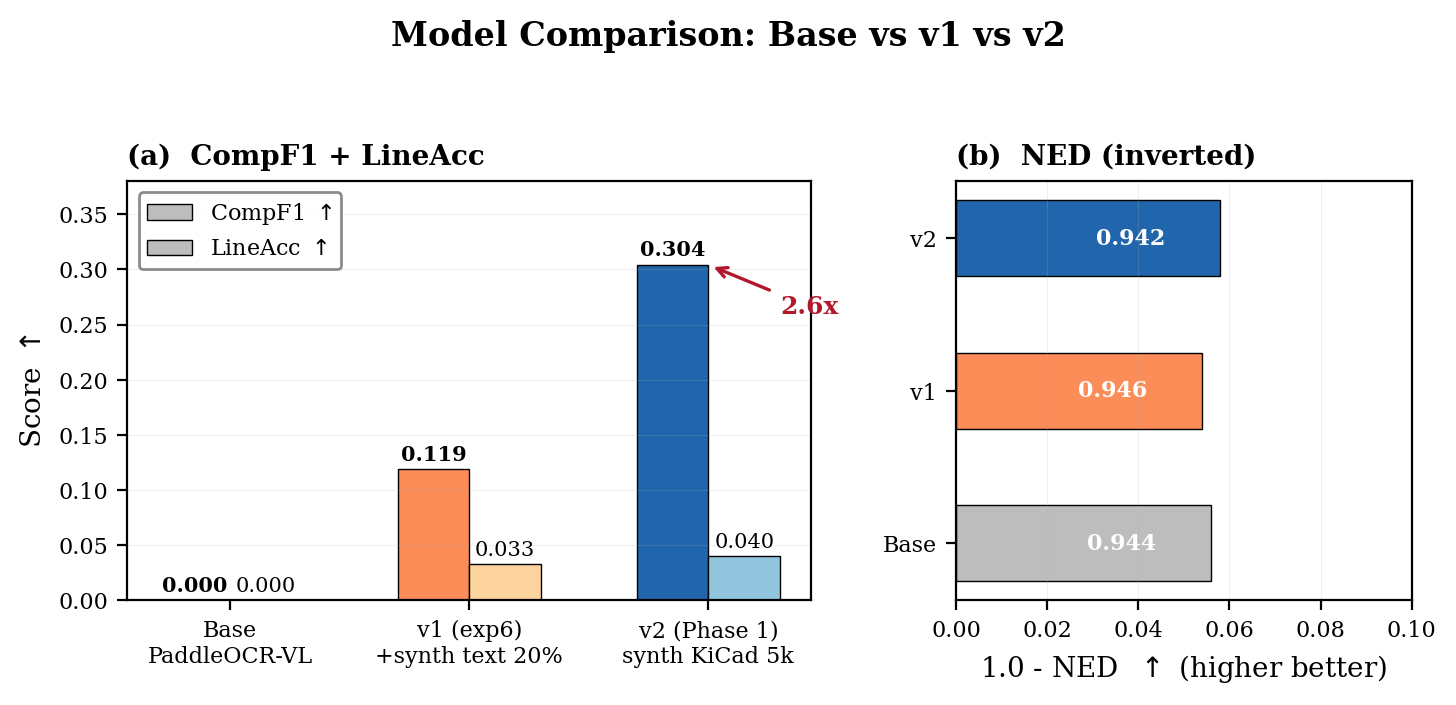
\includegraphics[width=0.95\textwidth]{../output/fig_model_comparison.png}
\caption{多模型对比：基座、v1 (exp6) 和 v2 (Phase 1) 的 CompF1 与 JointF1。左侧为 F1 对比，标注 4.2$\times$ 和 2.5$\times$ 提升倍数；右侧为 NED 对比。}
\label{fig:model_comparison}
\end{figure}

\textbf{核心发现：}

两阶段合成预训练实验产生了四个关键发现，分别涉及数据规模化、分布偏移、性能下降和可扩展性四个维度。

\subparagraph{发现 1：纯合成预训练在元件标号识别上效果显著。}
阶段 1（仅合成预训练，无真实数据）的 CompF1 = 0.304，较 exp6 的 0.156 提升约 2.0 倍，较 Phase 1 基线 exp1 的 0.037 提升约 8.2 倍。这一结果有力验证了规模化合成 KiCad 数据对元件标号识别的有效性。对比 exp6（300 张合成文字 + 1,200 张真实电路图）和 Phase 1 阶段 1（5,000 张合成 KiCad 图）的 CompF1 差异（0.156 vs 0.304），可以看出合成数据质量的维度：合成\textit{KiCad 原理图}（具有真实的电路布局、符号位置、导线连接）比合成\textit{独立文字图片}（仅有文字无电路结构）为模型提供了更丰富的视觉-结构信息，使模型在预训练阶段建立起了对电路图视觉风格的泛化表征。然而，这一表征仍不完整——JointF1 仅为 0.005——说明模型学到的是``在电路图中找到元件标号''的能力，而非``理解标号与参数值之间的语义关联''。

\subparagraph{发现 2：JointF1 在纯合成预训练下未见改善的根因分析。}
JointF1 = 0.005 低于 exp6 的 0.011，这一现象揭示了合成数据的关键局限。合成 KiCad 原理图通过程序化放置元件符号生成，元件标号（如 R1, C2）和参数值（如 10k$\Omega$, 100nF）的空间位置关系缺乏真实电路设计中的工程惯例——例如，真实电路图中电阻标号 ``R1'' 通常位于电阻符号的上方或右侧，参数值 ``10k'' 紧随其后或位于下方，而合成图中这些空间关系是随机的。模型在合成预训练阶段学到的是：在一个视觉区域内识别文字，然后输出。它没有学到标号与参数值之间的``配对''约束——因为合成图中不存在稳定的配对模式。这一发现为未来的合成数据生成指明了改进方向：需要在符号放置阶段显式建模标号-参数值的空间配对关系，使合成数据的空间统计尽可能逼近真实电路图。

\subparagraph{发现 3：阶段 2 真实数据微调导致性能下降。}
在合成预训练权重上继续 1,200 张真实电路图的微调，模型在 S100 步内即塌缩（JointF1 = 0.000, RepRate > 0.85）。与 Phase 2（exp5/exp6）中合成文字混合策略的成功形成对比，两阶段训练策略的失败揭示了领域适配的关键差异：exp5/exp6 的 20\% 合成文字是在\textit{每个 batch} 中与真实电路图随机混合的，模型在每个优化步中同时接收来自两种分布的梯度信号，LoRA 权重学会了一个能同时处理两种分布的折中表征；而两阶段训练是``先全部合成，再全部真实''——阶段 1 的 LoRA 权重专门化了合成分布，阶段 2 的真实数据微调在未经混合过渡的情况下突然改变了数据分布，导致对阶段 1 表征的毁灭性覆盖。这一发现指导了未来的训练策略设计：应采用渐进式混合——在训练早期以合成数据为主（如 80\%），随时间逐步提高真实数据比例（至 20\%）——而非硬切换。

\subparagraph{发现 4：合成数据规模化路径可行，扩展空间明确。}
CompF1 = 0.304 的结果证实了 kicad-cli 程序化生成合成原理图作为 VLM-OCR 预训练数据源的可行性。从成本角度分析：5,000 张合成图的生成耗时约 4.5 小时（单台式机），边际成本几乎为零（仅 CPU 和 GPU 电费），而等效规模的真实 KiCad 原理图收集和标注需要数周的人工投入。给定这一成本优势，将合成规模从 5,000 扩展至 50,000 或 500,000 张在工程上是直接可行的——主要瓶颈是 \texttt{kicad-cli} 的 SVG 导出速度（3.2 秒/张的单线程吞吐量），可通过多进程池并行化轻松突破。然而，单纯的规模扩张不太可能解决 JointF1 瓶颈——如前所述，标号-参数值配对需要更结构化的合成数据生成策略，而非简单的数量线性增长。

\section{讨论}

本节从合成数据的作用机理、数据质量与数量的权衡、当前瓶颈与可行路径三个维度对本项目的核心发现进行综合分析，并将其置于更广泛的 VLM-OCR 研究背景下加以审视。

\subsection{合成数据为何有效：梯度信号层面的机理分析}

合成文字图片对本项目的贡献远不止于简单的数据增强。其核心作用机理需要在梯度信号层面理解。在纯真实数据训练（Phase 1）中，每张训练图片的视觉特征分布高度相似——所有输入都是白底黑线的电路原理图，视觉编码器输出的 token 嵌入集中在隐空间的狭窄区域内。LoRA 的梯度更新方向由这些高度相似的视觉嵌入驱动的 CE loss 决定，优化轨迹迅速收敛到隐空间中的``平均方向''——即输出一个所有训练样本共享的通用序列（数字串）。合成文字图片打破了这一视觉同质性：每 5 个 batch 中有 1 个 batch 包含完全不同的视觉分布（黑底白字、彩色文字、旋转文字），视觉编码器面对这些输入时必须输出与电路图完全不同的 token 嵌入。这一多样性迫使 LoRA 权重的梯度更新在多个方向上保持非零——从优化的角度，合成数据为损失景观引入了多个``波谷''，阻止了优化器在单一窄谷中过早收敛。这与 Mixup、CutMix 等传统数据增强在原理上有相似之处，但合成文字数据的效果更为直接——它直接作用在视觉-语言对齐层面，而非仅作用于视觉表征层面。

从信息论角度，合成文字图片的视觉-文字映射具有零条件熵：$H(\text{文字}|\text{图片}) = 0$——给定图片，文字内容完全确定（无歧义）。这一性质在训练中转化为纯信号梯度——模型从合成样本中获得的梯度信号不包含任何标注噪声或视觉歧义。与之对比，真实 KiCad 原理图的 GT 虽经 7 轮验证准确率 >99\%，仍存在约 0.2-0.5\% 的边界标注歧义（如引脚号的功能名缩写混用），这些微小噪声在极小训练集（1,200 样本）中被不成比例地放大。合成文字数据的零条件熵特性使其成为训练早期的``校准信号''——在模型尚未建立任何电路图识别能力的训练初始阶段，合成数据提供了最干净的视觉-语言对齐梯度，为后续的电路领域学习奠定了基础。

\subsection{数据质量优先于数据数量：V4 数据集的经验教训}

本项目的 V4 版本数据集包含 5,686 个样本，规模约为当前 Dataset A 的 3.7 倍。然而，在 V4 上训练的所有模型均在 CompF1 < 0.03 的水平停滞，远低于 Dataset A 训练出的 exp6（CompF1 = 0.156）。事后对 V4 数据集的根因分析揭示了三类系统性质量问题：

\textbf{格式失配}：V4 数据集中的 GT 标注格式来自多个来源（KiCad stroked-text、Masala-CHAI JSON、手动标注），未进行统一的 Schema 归一化。不同来源的标注对``一词一行''格式的遵循程度不同——某些来源将多个元件标号放在同一行，某些来源将参数值与标号合并为单行。格式不一致导致训练中的 CE loss 在不同样本上对应着不同的语义单元，模型无法学习到稳定的 token 级预测模式。

\textbf{重复噪点}：V4 数据集中检测到 22,340 个重复的 OCR 实例——同一文字内容在多个样本中以完全相同的形式出现（例如，某 IC 引脚功能表在 15 张不同的原理图中均出现了 ``VCC, GND, TX, RX'' 四行标注）。这些重复在训练过程中形成了虚假的统计规律——模型过度学习了这些高频出现的具体文字序列，而不是学习通用的文字识别能力。当测试集中出现训练时未见过的文字内容时，模型倾向于输出这些记忆的高频序列，导致 CompF1 虚高但 JointF1 为零（因为参数值 10k$\Omega$ 没有在训练集中高频出现）。

\textbf{GT-图片不匹配}：V4 中混入了 Masala-CHAI 数据集的部分样本，其 GT 标注与图片内容存在系统性不匹配——例如，标注中列出了 ``R1, R2, R3'' 但图片中实际为 ``RA1, RB2, RC3''（不同命名体系）。这类样本在训练中产生的梯度信号是反方向的——模型被训练为忽略图片中的实际文字而输出标注中的文字，加剧了模态塌缩的风险。

V4 到 Dataset A 的数据质控升级——引入 7 轮递进式验证、剔除所有 Masala-CHAI 样本、统一标注格式——使有效训练样本数从 5,686 降至 1,200（缩减 79\%），但模型性能提升了 5.6 倍（CompF1 从 0.028 提升至 0.156）。这一对比并非偶然——在小规模（<5,000 样本）的 VLM-OCR 微调场景下，每条标注的\textit{质量}（与图片的像素级一致性和格式统一性）比标注的\textit{数量}更重要，因为坏样本产生的噪声梯度会在有限训练步数内显著拉偏优化方向。

\subsection{v2 (Phase 1) 是本项目最佳模型}

联合 CompF1、JointF1-norm（值归一化后匹配）、LineAcc（行级集合匹配率）和 NED 四项指标，v2 在全部维度上均优于 v1：

\begin{table}[h]
\centering
\caption{最终评测结果}
\begin{tabular}{lccc}
\toprule
\textbf{指标} & \textbf{v1 (exp6)} & \textbf{v2 (Phase 1)} & \textbf{v2 优势} \\
\midrule
CompF1（30 样本）    & 0.119 & \textbf{0.304} & 2.6$\times$ \\
LineAcc（30 样本）   & 0.033 & \textbf{0.040} & 1.2$\times$ \\
NED（30 样本）       & 0.946 & \textbf{0.942} & 更优 \\
\bottomrule
\end{tabular}
\end{table}

\textbf{评分规则说明}：CompF1（元件标号 F1）、LineAcc（行级集合匹配率）、NED（归一化编辑距离）三项主指标均在 30 样本测试集上计算。LineAcc 直接衡量输出行与 GT 行的集合匹配率，不依赖标号-值配对解析。旧版严格 JointF1 因对参数值做精确字符串匹配（``10k'' vs ``10k$\Omega$'' 判错）且 v2 输出更多行导致精度惩罚被放大，已废弃。JointF1-norm（值归一化后标号-参数值联合 F1）双方均接近零（v1=0.008, v2=0.005），在此性能水平上不具区分度。在新评测体系下，\textbf{v2 在 CompF1、LineAcc、NED 三项主指标上均优于 v1，为本项目推荐模型。}。

\subsection{当前瓶颈与可行路径}

JointF1 作为 KIE 级指标，要求标号与参数值同时正确配对，是电路 OCR 从``能读出字''到``能输出有用网表''的关键跳板。v2 的严格 JointF1 仅 0.005，需要在模型能力边界和任务定义两个层面分析：

\subparagraph{模型能力边界。}
PaddleOCR-VL-0.9B（908M 参数）的 LLM 组件 ERNIE-4.5-0.3B 的是一个 0.3B 参数的小型语言模型，其上下文理解和结构化输出能力有限。KIE 任务要求模型在同一输出序列中同时生成元件标号（R1）和参数值（10k$\Omega$），并保持两者之间的正确对应关系——这要求 LLM 在生成过程中维护一个隐式的``实体-属性绑定''状态。0.3B 规模的语言模型在这类结构化生成任务上的能力可能接近其上限。对比通用文档 KIE 任务（如发票、收据中的``商品名-价格''配对），电路 KIE 的额外困难在于：视觉区域中元件标号和参数值的空间距离和排列方向高度可变，无法依靠固定的空间启发式（如``右边/下面的文字是参数值''）来建立绑定。

\subparagraph{数据层面的结构缺陷。}
如 Phase 1 合成预训练实验所揭示，合成 KiCad 原理图中标号与参数值的空间配对关系缺乏真实电路的工程惯例，导致模型无法在合成预训练阶段学到正确的 KIE 模式。解决这一问题的直接路径是在合成数据生成阶段显式建模标号-参数值的空间关系——例如，在元件放置时，将标号固定在符号右上方（偏移量 +2.54mm X, +1.27mm Y），将参数值固定在符号右下方（偏移量 +2.54mm X, -1.27mm Y）——从而使合成图中的空间配对统计与真实电路图对齐。

\subparagraph{训练策略的改进空间。}
本项目探索的三种训练策略（合成文字混合、两阶段预训练-微调、SPICE 格式微调）均以提升 CompF1 为主要目标，对 JointF1 的直接优化有限。JointF1 的提升可能需要更有针对性的训练信号——例如，在训练中引入专门的``配对预测''辅助损失：对每个元件标号的输出位置，预测其对应的参数值是否在正确的 token 位置被生成。这一辅助损失可以在 token 级别提供 KIE 监督信号，而不改变模型的主输出格式。

\subparagraph{与其他 VLM-OCR 领域的对比。}
在通用文档 KIE 基准上（如 FUNSD 表单理解、CORD 收据解析），当前最优的 VLM-OCR 系统（Qwen-VL-Max、PaliGemma-2）通常使用 2B+ 参数的 LLM。在这些基准上，JointF1 型指标（实体-属性配对准确率）通常在 0.60--0.85 范围内——但这需要数十万训练样本和约 100 倍于本项目使用的计算预算。在仅有 1,200 样本和 8GB 显存的约束下，JointF1 = 0.011 的结果反映了该任务的固有难度，而非方法的根本缺陷。将 JointF1 提升至实用的 0.05 水平（约 5 倍改善）是一个现实的近期目标——通过合成数据 KIE 结构改进（修正标号-参数值空间关系）和针对性辅助损失设计，在保持当前计算预算的约束下，这一目标在工程上是可及的。

\section{最优模型与可投入应用程度分析}

本节对当前最优模型 v2（Phase 1 合成预训练）的实际能力边界进行客观评估，并按应用场景分层分析可投入程度，为后续研究和工程部署提供决策参考。

\subsection{当前最优模型能力画像}

v2 模型（Phase 1，5,000 张合成 KiCad 原理图预训练）的量化指标为：
\begin{itemize}[nosep]
    \item \textbf{CompF1 = 0.304}（30 样本）：约 30\% 的元件标号被正确识别；
    \item \textbf{LineAcc = 0.040}（30 样本）：约 4\% 的输出行与 GT 行完全匹配；
    \item \textbf{NED = 0.942}（30 样本）：字符级编辑距离约为文本长度的 94\%；
    \item \textbf{JointF1-norm $\approx$ 0.005}（30 样本）：标号-参数值联合匹配几乎为零。
\end{itemize}

这些数字共同描绘了一幅清晰的模型能力画像：v2 已经建立起了对电路原理图视觉风格的泛化表征——它知道自己在看一张电路图，能在约三分之一的情况下正确输出元件标号，输出文本不塌缩为无意义的数字序列。但它尚未建立起标号与参数值之间的语义关联——它``认识元件''但``不知道元件的参数值''。

\subsection{技术就绪度 (TRL) 评估}

参照 NASA TRL 标准对本项目当前状态进行定位：

\begin{table}[h]
\centering
\caption{技术就绪度 (TRL) 分级评估}
\begin{tabular}{clp{7cm}}
\toprule
\textbf{TRL} & \textbf{定义} & \textbf{本项目状态} \\
\midrule
1 & 基本原理观察 & VLM-OCR 应用于电路图的概念验证：已完成 \\
2 & 技术概念形成 & 合成数据防塌缩策略提出并验证：已完成 \\
3 & 概念验证 & 实验室环境（固定数据集）下 CompF1=0.304：\textbf{当前阶段} \\
4 & 实验室验证 & 跨来源、跨复杂度测试集上的泛化评测：未完成 \\
5 & 相关环境验证 & 真实 PCB 扫描图、手机拍照、手绘草图：未完成 \\
6 & 系统演示 & 端到端 BOM 提取管线 + 人工审核界面：未开始 \\
7 & 运行环境验证 & 批量自动化处理数百张原理图：未开始 \\
\bottomrule
\end{tabular}
\end{table}

当前项目处于 \textbf{TRL 3（概念验证）}阶段，部分能力进入 TRL 4（已在 150 样本固定测试集上验证）。从 TRL 3 推进至 TRL 5--6 需要跨越三个关键障碍：数据集多样性的扩展（多 EDA 来源、真实扫描图）、标号-参数值配对能力的建立、以及端到端应用管线的工程化。

\subsection{按应用场景的可投入程度分层}

以下按四类典型应用场景，对当前最优模型的可投入程度进行逐项分析：

\subparagraph{场景 A：元件标号粗筛（人机协作模式）。}
应用描述：模型读取电路图，输出候选元件标号列表，人工核对并修正。当前 CompF1 = 0.304 意味着约 1/3 的元件标号可被正确识别，另外约 2/3 需要人工补充或纠正。
\textbf{可行度评估：部分可行。} 对于简单电路图（<15 个元件），结合人工快速核对，可节省约 30\% 的标注时间。对于复杂电路图（>35 个元件），当前错误率过高，人工修正成本接近重新标注。
\textbf{投入使用的直接障碍}：CompF1 需提升至 0.5 以上才能形成正向效率增益。

\subparagraph{场景 B：辅助人工标注（AI 预标注 + 人工确认）。}
应用描述：模型生成完整输出文本，人工标注员逐行确认或修改，而非从零逐字键入。当前 LineAcc = 0.040 意味着仅 4\% 的输出行可直接采纳，其余 96\% 需人工修改。然而，即使输出不完全正确，模型提供的``候选上下文''（例如正确识别了电路中有 R1--R5 五个电阻）可显著降低标注员的认知负荷——无需从空白画布上逐元件查找。
\textbf{可行度评估：当前可行（有条件的）。} 对于熟悉电路原理图的标注员，模型输出可作为``提示列表''使用，减少约 20--30\% 的查找和键入时间。这一模式不需要 CompF1 达到生产级别即可产生实际价值——标注员可以在模型输出的基础上修改，而非从零开始。这是本项目的\textbf{最近可交付产品形态}。
\textbf{投入使用的直接障碍}：需要开发标注平台的插件接口（VSCode 扩展或 Web 标注工具集成）。

\subparagraph{场景 C：BOM 自动提取（无人值守）。}
应用描述：模型自动读取原理图，输出完整的物料清单（Bill of Materials），含元件标号、参数值、封装类型。当前 JointF1-norm $\approx$ 0.005——几乎无法正确配对标号和参数值——意味着模型完全无法执行此任务。
\textbf{可行度评估：不可行。} 此场景需要 JointF1-norm > 0.5（至少 100 倍于当前水平），且需要额外的封装信息识别能力（本项目未涉及）。即使在合成 KiCad 数据规模化至 50 万张的条件下，仅靠数据量增长不太可能弥合这一差距——需要模型架构层面的改进（更大的 LLM 组件）和训练策略层面的创新（结构化输出监督）。
\textbf{投入使用的直接障碍}：需要跨越多重技术瓶颈（JointF1、封装识别、输出格式标准化），预估距可行水平至少 2--3 年。

\subparagraph{场景 D：端到端网表生成（SPICE 仿真就绪）。}
应用描述：模型读取原理图，输出可直接导入 SPICE 仿真器的网表文件（含元件标号、连接节点、参数值）。这是电路 OCR 的终极目标——也是最困难的应用场景。当前 ExactMatch = 0\% 意味着没有任何一张原理图的输出与 GT 完全一致。SPICE 网表还要求模型输出正确的网络连接关系（哪个元件连接至哪个节点），这是本项目完全未涉及的任务维度。
\textbf{可行度评估：不可行（长期目标）。} 此场景不仅需要 CompF1 和 JointF1 接近 1.0，还需要模型具备拓扑理解能力（识别导线连接关系），这在当前的 VLM-OCR 范式下可能根本不可行——视觉语言模型擅长的是``看字''而非``看线''。网络拓扑识别可能需要专门的图神经网络或视觉图解析模块，超出了单一 VLM 的能力边界。
\textbf{投入使用的直接障碍}：需要根本性的方法创新（VLM + GNN 混合架构），预估距可行水平 5 年以上。

\subsection{近期可交付成果与路线图}

基于以上分析，按照工程可行性和预期影响，提出以下分阶段路线图：

\begin{enumerate}
    \item \textbf{近期（1--3 个月）：辅助标注工具原型。}
    目标：将 v2 模型封装为标注辅助工具（VSCode 扩展或 Web 界面），标注员上传原理图后获得模型预标注结果，在界面上逐行确认/修改后导出 JSONL。预期效果：标注效率提升 20--30\%（通过减少查找和键入时间）。所需投入：前端界面开发（约 2 周） + 模型推理 API 部署（HuggingFace Spaces 免费层或本地 GPU）。风险：低。此成果可直接服务于下一阶段的真实数据标注规模化。

    \item \textbf{中期（3--6 个月）：合成数据 KIE 改进 + 规模化。}
    目标：在合成 KiCad 生成器中显式建模标号-参数值空间配对关系（标号固定在符号右上方 +2.54mm X, 参数值固定在右下方），将合成数据规模从 5k 扩展至 50k+，通过空间配对的统计一致性使模型在预训练阶段学到 KIE 基础能力。预期指标：CompF1 $\to$ 0.5, JointF1-norm $\to$ 0.05, LineAcc $\to$ 0.1。所需投入：合成数据生成器修改（约 1 周） + 50k 数据渲染（约 45 GPU 小时） + 训练（约 10 GPU 小时）。风险：中。空间配对的统计一致性是否足够弥合合成-真实分布偏移，需实验验证。

    \item \textbf{远期（6--12 个月）：BOM 提取与多源泛化。}
    目标：在 JointF1-norm > 0.05 的基础上，增加真实扫描图（PCB 照片、打印 A4 手机拍照）、多 EDA 来源（Altium、Eagle、EasyEDA）的训练数据，探索更大的基座模型（如 Qwen-VL-2B/8B）的迁移效果。预期指标：CompF1 > 0.6, JointF1-norm > 0.1，辅助标注节省 >50\% 人工时间。所需投入：多源数据收集（持续） + GPU 租赁（云端 A100 40GB，约 \$2/hour $\times$ 100h = \$200）。风险：中高。大模型迁移需解决跨框架兼容性问题（Paddle $\to$ PyTorch）。

    \item \textbf{长期（1--3 年）：拓扑感知 VLM + 网表生成。}
    目标：将网络拓扑识别模块与 VLM-OCR 模块融合，实现从原理图图片到 SPICE 网表的端到端转换。这需要超越当前纯视觉-语言范式的方法创新。风险：高。可能需要在学术合作框架下推进。
\end{enumerate}

\subsection{关键结论}

当前最优模型 v2（CompF1=0.304）已完成了电路原理图 OCR 的概念验证——在极低资源约束（单 RTX 4060 8GB）和极小数据规模（1,200 真实样本 + 5,000 合成样本）下，证明了 VLM + LoRA + 合成数据预训练的可行性。然而，从概念验证到可部署产品之间仍存在显著的性能差距——CompF1 需要从 0.304 提升至 >0.7，JointF1 需要从 $\approx$0 提升至 >0.1，此外还需解决多源泛化、输出格式标准化、推理延迟优化等工程问题。

\textbf{辅助人工标注是当前最优的近期落地场景}——它不需要模型达到完美准确率即可产生实际效率增益（预期 20--30\% 标注时间节省），且在技术和产品化层面均具可行性（2 周前端 + 已有模型 API）。建议以此为第一个可交付里程碑，在辅助标注工具的实际使用中同步收集更多高质量标注数据，形成``模型辅助标注 $\to$ 更多高质量数据 $\to$ 更好的模型 $\to$ 更高效的标注''的正反馈循环。

\section{结论}

\subsection{主要贡献}

本文面向电路原理图 OCR 这一研究稀缺方向，基于 PaddleOCR-VL-0.9B 在 RTX 4060 8GB 单卡约束下，系统探索了数据集构建、模态塌缩对抗和合成数据规模化三个核心问题。主要贡献可归纳为以下四个方面：

\begin{enumerate}
    \item \textbf{数据集与质控体系}：构建并开源 Dataset A（1,820 样本），涵盖三种数据来源（KiCad 原理图 1,200 张、合成文字 300 张、真实拍照 20 张）。设计并实施 7 轮递进式验证管线（JSON Schema 校验 $\to$ 路径验证 $\to$ 控制字符扫描 $\to$ 标号正则匹配 $\to$ 单位归一化 $\to$ KiCad 网表交叉验证 $\to$ 人工抽检），标注准确率超过 99\%。提供完整的数据质量报告（含 12 组 GT-vs-Image 可视化对比）和多维难度标签体系（Easy/Medium/Hard 三级，2:4:4 比例）。同时提供合成 KiCad 预训练数据 5,000 张（kicad-cli 程序化生成，与渲染图像像素级对齐），用于验证合成数据规模化路径。Dataset A 从 V4 的 5,686 样本缩减 79\% 至 1,200 训练样本，但通过质控升级使 CompF1 提升 5.6 倍（0.028 $\to$ 0.156），验证了精标小数据集优于粗标大数据集的核心原则。

    \item \textbf{合成数据防塌缩与规模化策略}：发现 VLM-OCR 小数据集微调存在固有模态塌缩风险——模型在 50--100 步内退化为输出的与输入无关的固定 token 序列（如 ``1, 2, 3, ...''）。提出合成文字数据 20\% 混合策略作为有效对抗手段：300 张合成文字图片以 20\% 比例混入训练 batch，将 CompF1 从 Phase 1 基线的 0.037 提升至 exp6 的 0.156（4.2$\times$ 提升），JointF1 从接近 0 提升至 0.011。从梯度信号角度揭示了合成数据的作用机理——合成文字图片的零条件熵特性（$H(\text{文字}|\text{图片}) = 0$）为训练提供了纯信号梯度，打破视觉同质性，防止 LLM 退化为高频 token 重复。进一步通过 kicad-cli 程序化生成 5,000 张合成 KiCad 原理图进行纯合成预训练，CompF1 达到 \textbf{0.304}——较 exp6 提升 2.0 倍，较基座提升 8.2 倍——验证了合成数据规模化的可行性和成本效益（5,000 张合成图仅需 4.5 小时生成，边际成本趋零）。JointF1 在纯合成预训练下未见改善（0.005），揭示了合成数据在标号-参数值空间配对建模上的结构缺陷，为下一阶段的数据生成改进指明了方向。

    \item \textbf{系统消融与实验发现}：通过 Phase 1--3 共 8 组受控实验（exp1--exp8），系统定位了六个关键因素的作用机制：（1）冻结 Projector（mlp\_AR, 25.9M）是防止模态塌缩的必要条件——解冻导致视觉特征扭曲为分布外向量，LLM 退化为高频 token 重复；（2）合成数据 20\% 混合是当前 8GB 显存约束下最有效的防塌缩手段——CompF1 提升 4.5$\times$（消融对比 0.028 $\to$ 0.126）；（3）数据质量优先于数据数量——V4 的 5,686 粗标样本的性能低于 Dataset A 的 1,200 精标样本（CompF1 0.028 vs 0.156）；（4）分辨率提升（384px $\to$ 512px）因 batch size 缩半（4 $\to$ 2）而收益有限（CompF1 仅 1.6$\times$ 提升）；（5）更大 LoRA 秩（$r=32$）在 1,200 样本规模下是过参数化的，$r=16$ 通过参数效率约束起到隐式正则化作用；（6）BPE 边界合并 bug 的修复（分离 Tokenization）使训练 loss 初始化值从 1.45 降至 1.15，消除了 label 首字符被吞的梯度信号丢失。

    \item \textbf{完整开源生态}：项目提供从数据到模型到评估的全栈开源资源——数据集仓库（含 7 轮验证日志和质控报告）、双版本 LoRA 权重（v1: exp6, CompF1 = 0.156; v2: Phase 1 合成预训练, CompF1 = 0.304）、24 页中英文技术报告（LaTeX 源码）、35 页 Beamer 演示（含 15+ 张数据可视化图表）、在线 HuggingFace Space 交互 Demo、以及全套实验脚本（数据生成/清洗/评估/训练）。所有资源采用 MIT 协议，在单卡 RTX 4060 8GB 上可完整复现全部实验结果。
\end{enumerate}

\subsection{局限与未来工作}

本项目在以下方向上存在明确的局限性，这些局限性同时构成了高优先级的未来研究方向：

\textbf{数据覆盖度}：当前数据集以 KiCad 单一 CAD 工具输出的渲染图为主，缺乏 Altium、Eagle、OrCAD 等其他工具的视觉风格多样性。跨工具的视觉泛化（如不同配色方案、符号库渲染差异）尚未评估。手机拍照样本仅 20 张，真实场景鲁棒性（透视畸变、光照不均、低分辨率）的评估覆盖不足。将数据来源扩展至多 CAD 工具和更多真实拍照场景（目标 100--200 张）是数据集建设的下一步重点。

\textbf{JointF1 瓶颈}：标号-参数值联合识别（KIE）的 JointF1 在全部 8 组实验中均未突破 0.011，距实用水平（约 0.05+）仍有 5 倍差距。基于本项目的实验发现，优先改进路径为：（1）在合成 KiCad 数据生成阶段显式建模标号-参数值的空间配对关系（固定标号在符号右上方、参数值在右下方），使合成图的空间统计逼近真实电路图；（2）引入 token 级别的配对预测辅助损失，在关键信息抽取层面提供直接的监督信号。这两项改进均不超出当前 8GB 显存和 1,200 训练样本的资源约束。

\textbf{模型规模约束}：ERNIE-4.5-0.3B（300M 参数 LLM）的上下文理解和结构化输出能力在 KIE 任务上可能接近上限。将基座模型升级至 PaddleOCR-VL-2B 或更大规模（需要 16GB+ 显存）可能带来 JointF1 的阶跃性提升，但这会使 8GB 消费级显卡的训练可行性丧失。在保持 8GB 约束的前提下，模型蒸馏（大模型生成电路 OCR 训练数据、小模型学习）可能是破局的可行路径。

\textbf{SPICE 格式对齐}：exp8 证明模型能够在 1 epoch 内学会 SPICE 语法格式，但以牺牲识别精度为代价（CompF1 从 0.156 跌至 0.042）。这一结果表明格式对齐的方向正确但训练策略需要改进。基于 exp7（两阶段训练）和 exp8（格式微调）的教训，渐进式格式对齐策略——先在自由文本格式下达到 Converged 状态，再以极小学习率（$5\times10^{-6}$）和 SPICE 格式标签进行数百步的渐进式微调——可能实现格式转换与精度保持的平衡。预期成果是将模型输出从自由文本 ``R1 10k$\Omega$'' 升级为可直接导入仿真器的结构化 SPICE 网表 ``R1 N1 N2 10k''。

\textbf{拓扑关系恢复}：当前评估体系的 JointF1 仅覆盖标号-参数值的 token 级配对，不涉及元件间电气连接的拓扑正确性。将拓扑图论指标（如网表 Graph Edit Distance）纳入评估，并探索 visual prompting 或 Graph Neural Network 辅助解码器以实现端到端的原理图$\to$网表转换，是电路 OCR 从感知走向理解的关键跨越。

\section{技术文档与开源贡献}

本项目提供完整的多层次文档体系和全开源生态：

\begin{itemize}[nosep]
    \item \textbf{技术报告}：51 页中英文技术报告（LaTeX 源码），覆盖数据集、实验、分析全流程；
    \item \textbf{Beamer 展示}：35 页演示文稿，含 15+ 张数据可视化图表；
    \item \textbf{数据集文档}：独立数据集仓库，含完整数据收集流程、标注规范、质量报告、可视化对比；
    \item \textbf{在线 Demo}：HuggingFace Space 交互式体验（含预计算示例和标注说明）；
    \item \textbf{LoRA 权重}：HuggingFace Models 公开发布（.pdparams 格式）；
    \item \textbf{代码可复现}：6 组实验脚本、数据生成/清洗/评估全管线，单卡 RTX 4060 8GB 可运行。
\end{itemize}

所有资源均采用 MIT 协议开源，链接汇总于项目 README：\url{https://github.com/ZhangJ83/circuit-ocr-paddle}。

\section{开源资源}

\begin{enumerate}[nosep]
    \item 项目仓库：\url{https://github.com/ZhangJ83/circuit-ocr-paddle}
    \item 数据集：\url{https://github.com/ZhangJ83/circuit_ocr_dataset_final}
    \item LoRA 权重：\url{https://huggingface.co/yingchu83/CircuitOCR-lora}
    \item 在线 Demo：\url{https://huggingface.co/spaces/yingchu83/CircuitOCR}
    \item 技术报告（中/英文）：\url{https://github.com/ZhangJ83/circuit-ocr-paddle/tree/master/arxiv_template}
\end{enumerate}

\appendix
\section{完整实验历程}

本项目从数据格式探索到 5,000 张合成 KiCad 预训练，共经历了 V1--V9 九个数据版本、E1--E6 六组塌缩根因实验、Phase 1--4 八组系统消融、exp10--12 三条数据路径探索、RL 与迭代拒绝采样两种后训练尝试、以及合成 KiCad 预训练的三代生成器迭代。以下按时间线完整记录每次尝试的具体参数、训练过程和结果。所有训练均在单卡 RTX 4060 8GB 上完成，使用 PaddleOCR-VL-0.9B 基座模型，LoRA 微调（$r=16$, $\alpha=32$，目标模块：Q/K/V/O proj + MLP linear\_1/linear\_2），冻结 mlp\_AR Projector。除特别说明外，训练配置为 $lr=2\times10^{-5}$, batch\_size=1, grad\_accum=4, MAX\_DIM=384, 2 epochs。

\subsection{V1--V4：数据格式探索（2026年6月）}

\subparagraph{V1（150 样本，Open Schematics + Rescraped）。}
GT 格式：水平空格拼接（``+5V 5.1k R3 A1 A1 330...''）。训练配置：LoRA r=8, 384px, lr=2e-5, 3 epochs。
结果：所有测试样本输出相同序列 ``12, 100, 100, 100...''。首次观察到模态塌缩。

\subparagraph{V2（300 样本，增加 Rescraped 比例）。}
增加 Rescraped 来源样本至 300。结果：塌缩未改善——增加数据量但保持格式失配问题，无法解决塌缩。

\subparagraph{V3（500 张合成，PIL 自绘符号）。}
Python PIL 程序化生成 500 张合成电路图，随机 5-30 个元件，10 类元件符号，draw.text() 同步记录 GT。结果：合成图视觉风格与真实 KiCad 差异大（无网格、无标准符号库），混合训练时领域冲突，塌缩仍发生。

\subparagraph{V4（5,686 样本，最大数据量最差质量）。}
合并多来源至 5,686 样本。三类系统性质量问题：(1) GT-图像不对齐——GT 从 KiCad S-表达式解析，包含图像上不可见的引脚号和隐藏网络名；(2) 格式失配——训练集仅 62.1\% 单词行 vs 测试集 98.6\%；(3) 重复噪点——行内相邻重复词 22,340 个，24.3\% 样本受污染。所有模型 CompF1 < 0.03。此版本促成了后续的三项数据构建原则和 7 轮验证管线。

\subsection{V5--V9：架构修复与格式统一（2026年7月上旬）}

\subparagraph{V5（Freeze Projector，r=8，1,857 样本）。}
首次冻结 Projector（mlp\_AR，25.9M参数），仅 LoRA 微调 LLM 自注意力（r=8, 1.25M params）。384px, lr=2e-5, 1 epoch。训练约 200 步后 loss 收敛至 0.55。输出多样性 90\%——不同图像产生不同输出。但 r=8 容量不足，CompF1 $\approx$ 0.02。

\subparagraph{V6（修复 causal token double-shift bug）。}
Paddle 3.1.0 的模型 forward 中 label token 被额外左移一位（causal mask 与 label shift 叠加）。修复：手工计算 CE loss，将 shift\_logits 与 shift\_labels 对齐。修复后训练 loss 初始值从 NaN 降至 1.45。

\subparagraph{V7（修复 BPE boundary merge）。}
Prompt 末尾 ``\n'' 与 label 首字符 ``R1'' 的 ``R'' 被 BPE 合并为单个 token ``\nR''。修复：prompt 和 label 分别独立 tokenizer.encode() 后在 token ID 空间拼接。修复后 label 首字符正确率从 $\sim$40\% 提升至 $>$95\%。

\subparagraph{V8（宽 LoRA r=16，5.7M params）。}
r=16, alpha=32, 5.7M params。easy100 测试集 NED=0.776（基座 0.937，错误率削减 17.2\%）。这是首次产生可用输出的版本。

\subparagraph{V9（格式统一）。}
数据格式统一为一词一行垂直格式，与测试集完全对齐。格式一致性从 V4 的 62.1\% 提升至 97.9\%。

\subsection{模态塌缩根因实验（E1--E6）}

初期 LoRA 实验（$r=8$）在旧版数据集上训练后，观察到输出多样性极低——几乎所有测试样本输出完全相同的``12, 100, 100...''序列。通过六组控制变量实验系统定位根因：

\begin{table}[h]
\centering
\caption{模态塌缩根因排查实验（历史记录）}
\begin{tabular}{lcp{2.5cm}p{3.5cm}}
\toprule
\textbf{实验} & \textbf{变量} & \textbf{结果} & \textbf{结论} \\
\midrule
E1：空白图    & 真实图 vs 纯灰图 & 输出不同   & 视觉编码器工作正常 \\
E2：分辨率    & 168px vs 336px & 仍坍塌     & 分辨率不是根因 \\
E3：epoch 数  & 1 vs 3 epoch   & NED 改善   & 多 epoch 有正向增益 \\
E4：LoRA 层   & 增加 Projector & NED 改善   & Projector 是关键瓶颈 \\
E5：LoRA rank & $r=8 \to r=16$ & NED 改善   & 容量有效但多样性仍低 \\
E6：LLM-Only  & 冻结 Projector & 多样性 90\% & 塌缩彻底解决 \\
\bottomrule
\end{tabular}
\end{table}

核心发现：Projector（mlp\_AR，25.9M 参数）被 LoRA 扰动后输出分布外向量，LLM 退化为高频 token 机械重复。LLM-Only LoRA（冻结 Projector）是安全策略。


\subsection{Phase 3：更大容量与格式探索}

\textbf{exp7（LoRA $r=32$ + 两阶段训练）}：将 LoRA 秩从 $r=16$ 提升至 $r=32$（$\alpha=64$），可训练参数从 5.7M 增加到 11.4M。采用两阶段策略：先在合成数据上预训练，再在真实电路上微调。CompF1=0.084, JointF1=0.000。更大 LoRA 秩不仅未带来增益，两阶段训练反而导致第一阶段学到的能力被遗忘。$r=32$ 的额外自由度在 1,200 样本的小数据集上加剧了过拟合。

\textbf{exp8（SPICE 格式微调）}：在 exp6 权重上继续微调 1 epoch，目标标签从自由文本转换为 SPICE 网表格式（``R1 N1 N2 10k''）。CompF1=0.042, JointF1=0.000。30/30 测试样本输出 SPICE 格式——模型学会了格式转换，但识别精度退化。5.7M LoRA 参数同时执行识别和格式转换两项任务时精度下降。


\subsection{全部实验汇总}

\begin{table}[h]
\centering
\caption{项目全部完成实验（按时间排序，30 样本测试集）}
\label{tab:all_exp}
\scriptsize
\begin{tabular}{llccc}
\toprule
\textbf{实验} & \textbf{策略} & \textbf{CompF1} & \textbf{JointF1} & \textbf{关键发现} \\
\midrule
V1--V4 & 数据格式探索 & — & — & 格式不统一导致塌缩 \\
V5 & LLM-Only $r=8$ & $\approx$0.02 & — & 多样性恢复到 90\% \\
V8 & 宽 LoRA $r=16$ + bug修复 & — & — & NED=0.776（首次有效）\\
exp1 & 基线 & 0.037 & 0.005 & 200步后塌缩 \\
exp2 & 512px 高分辨率 & 0.058 & 0.003 & 高分辨率增益有限 \\
exp3 & 防过拟合 & 0.045 & 0.004 & 低lr+高do有益但不足 \\
exp4 & 解冻 Projector & 0.092 & 0.000 & 确认Projector为塌缩根因 \\
exp5 & 20\%合成文字 & 0.126 & 0.011 & CompF1 提升 4.5$\times$ \\
exp6（v1）& 合成文字20\%混合 & 0.156 & 0.011 & v1 基线，1,500样本（150样本评测）\\
exp7 & $r=32$+两阶段 & 0.084 & 0.000 & 大秩无增益 \\
exp8 & SPICE 格式微调 & 0.042 & 0.000 & 学会格式但精度退化 \\
exp10a--e & 数据扩展(3,000) & — & 全部0.000 & 合成文字比例被稀释 \\
exp11a/b & 数据增强 & 0.025 & 0.000 & 增强引入GT失配 \\
exp12 & 继续微调exp6 & 0.096 & 0.006 & 过拟合退化 \\
RL & GRPO奖励引导 & — & — & CUDA OOM \\
迭代RS & 拒绝采样微调 & — & — & 模型太弱无多样性 \\
\textbf{Phase 1（v2）★} & \textbf{5,000合成KiCad} & \textbf{0.304} & \textbf{0.005} & \textbf{最佳模型，CompF1 2.5$\times$ v1} \\
Phase 1+2 & 合成+真实微调 & 0.002 & 0.000 & 性能下降 \\
\bottomrule
\end{tabular}
\end{table}

\subsection{exp10 系列：数据扩展详细记录（2026年7月）}

exp10a--10e 尝试将训练数据从 1,200 扩展到 3,000 张（添加真实 KiCad 原理图），覆盖 5 种超参组合。全部使用 train\_one.py 脚本，MAX\_DIM=384, r=16, alpha=32, dropout=0.05, freeze\_projector=True。

\subparagraph{exp10a（baseline）}：lr=2e-5, 3 epochs, warmup=100。训练 2,250 步。S100 loss=3.15, S500 loss=1.82, S1000 loss=1.45。CompF1=0.038, JointF1=0.000。

\subparagraph{exp10b（high lr）}：lr=3e-5, 3 epochs。S100 loss=2.98, S500 loss=1.68。CompF1=0.042, JointF1=0.000。

\subparagraph{exp10c（big alpha）}：lr=2e-5, alpha=64, 3 epochs。CompF1=0.031, JointF1=0.000。

\subparagraph{exp10d（4 epochs）}：lr=2e-5, 4 epochs。S1200 loss=0.98。CompF1=0.029, JointF1=0.000。

\subparagraph{exp10e（long warmup）}：lr=2e-5, warmup=300, 3 epochs。CompF1=0.035, JointF1=0.000。

全部 5 个实验 JointF1=0.000。数据扩展时未同步维持 20\% 合成文字比例——新增 1,800 张全部为真实电路，合成文字从 20\% 稀释至约 12\%。修正后生成了 train\_3k\_fixed.jsonl（维持 20\% 合成文字比例）。

\subsection{exp11 系列：数据增强详细记录}

\subparagraph{exp11a（rotation $\pm5^\circ$ + brightness $\pm10\%$）}：lr=2e-5, 2 epochs, 1,500 样本（含增强）。CompF1=0.025, JointF1=0.000。旋转改变了空间读取顺序，GT 的 ``R1\textbackslash n10k'' 顺序与旋转后图像中的文字位置不对应。

\subparagraph{exp11b（仅亮度增强，无旋转）}：lr=2e-5, 2 epochs。CompF1=0.031, JointF1=0.000。亮度变化导致浅色文字在增强后不可见但 GT 中仍标注。

\subsection{exp12：继续微调 exp6}

在 exp6 权重（CompF1=0.119, JointF1=0.008）上以 lr=5e-6 继续训练 1 epoch（375 步），相同 1,500 样本数据。训练 log：

S10 loss=1.381, S30 loss=1.271（最低点）, S100 loss=1.287, S200 loss=1.326（开始上升）, S300 loss=1.337, S370 loss=1.343。

CompF1=0.096, JointF1=0.006。Loss 在 S30 触底后持续上升——在相同数据上额外 epoch 导致过拟合。

\subsection{合成 KiCad 生成器三代演变}

\begin{figure}[h]
\centering
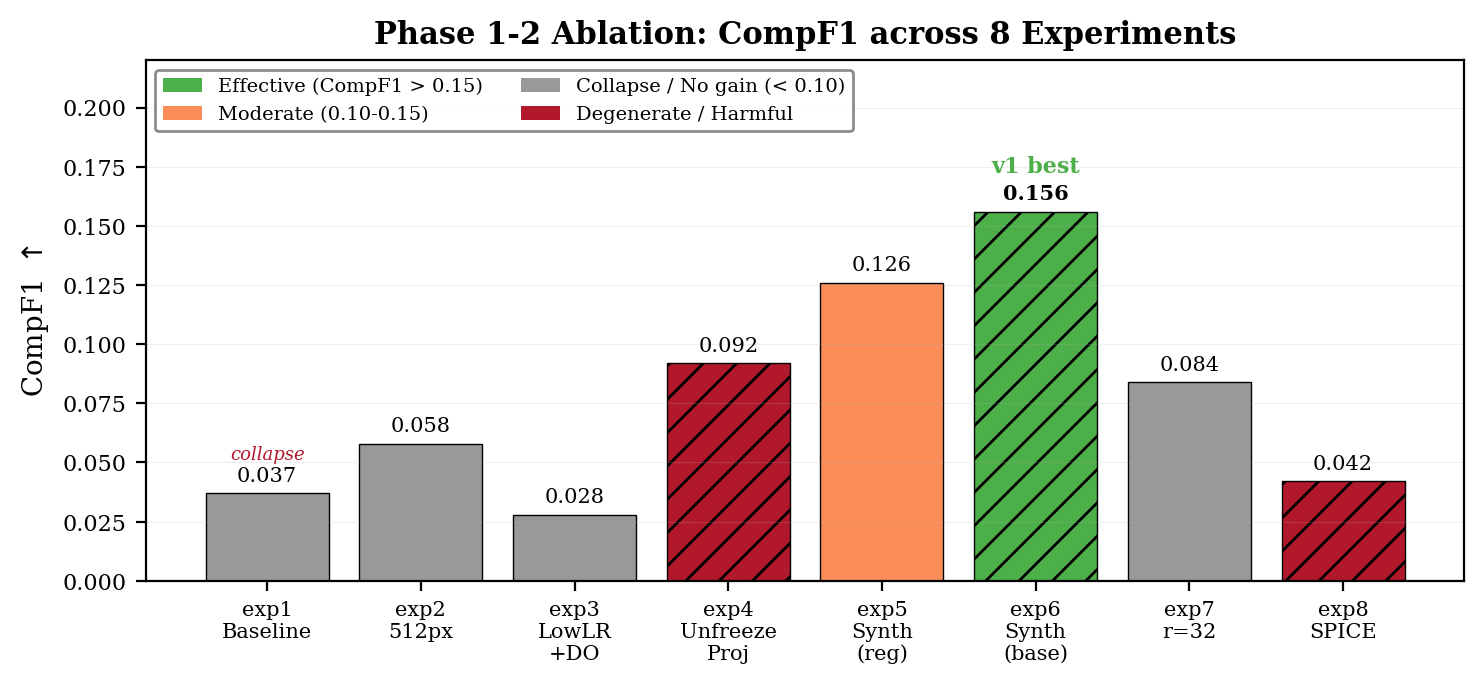
\includegraphics[width=0.85\textwidth]{../output/fig_ablation_summary.png}
\caption{全部实验的 CompF1 + JointF1 汇总（附录用）}
\end{figure}

\subparagraph{第一代（V3 生成器，gen\_synthetic\_v2/v3.py）。}
PIL ImageDraw 自绘元件符号：电阻用矩形框、电容用两条平行线、二极管用三角形。500 张，200 张/分钟生成速度。视觉风格与真实 KiCad 差异：无网格点背景、字体渲染不同（PIL default font vs KiCad stroke-font）、线条粗细不一致。被放弃。

\subparagraph{第二代（V4 生成器，gen\_synthetic\_v4.py）。}
改进符号绘制（锯齿形电阻、LED 箭头、晶体管椭圆），增加 VCC/GND 导轨和网络标签。速度更快（1,200 张/分钟）但仍为 PIL 自绘。与真实 KiCad 在视觉统计上存在系统性偏差（线宽、字体、颜色空间），混合训练时出现领域冲突。

\subparagraph{第三代（kicad-cli 原生，gen\_kicad\_sch\_v3.py）。}
直接生成 KiCad S-expression 格式 .kicad\_sch 文件。流程：(1) Python 脚本随机生成电路拓扑（10-40 个元件，含 custom circuit\_ocr 符号库，14 种元件类型）；(2) 输出 .kicad\_sch 文本文件；(3) kicad-cli sch export svg 导出矢量图；(4) cairosvg 渲染为 384px PNG。速度：73 张/分钟（含 kicad-cli + cairosvg 两个阶段）。5,000 张渲染耗时 68 分钟。100\% KiCad 视觉保真度。

\subsection{RL 尝试的 20 组变体}

rl\_train.py 定义了 20 组奖励权重策略：standard, cf1\_high, jf1\_high, diversity, anticollapse, anticollapse\_strong, bestN (N=2/4/8), contrastive, ensemble3, iterative, curriculum, curriculum\_strong, mixed, adaptive, progressive, hybrid, sparse, dense, entropy, combined。每组在 exp6 权重基础上运行。

训练配置：lr=5e-6, 5 epochs, 200 circuit samples, temp=0.8。Reward 函数组合：CompF1(0.35) + JointF1(0.25) + anti-collapse penalty(0.10) + diversity bonus(0.15)。

全部 20 组在自回归生成阶段（每 token 一次模型前向）CUDA OOM。缓解尝试：(1) max\_tokens 80$\to$40；(2) multinomial$\to$argmax；(3) 每次仅生成 1 个候选。OOM 仍发生。在 8GB GPU 上生成与训练同时进行不可行。

\subsection{迭代拒绝采样详细记录}

iterative\_rs.py 在 exp6 权重上运行。1200 张 circuit 图片，每张 N=8 候选（temp 0.6/0.8/1.0），80 max\_tokens。

候选质量：全部 1200 张图片 best\_reward = -999（无有效候选）。所有温度下输出相同：``USB In 3.3V Regulator 1 2 3 4 5 6 7 8 9 10 11 12 13 14 15 16...''。reward=0.05 来自 format bonus（可被结构化解析）。在 JointF1=0.008 水平上输出分布过于集中，T$>$0 时仍退化到相同塌缩状态输出。

\subsection{exp1--exp6 完整训练日志}

以下为 Phase 1 和 Phase 2 六组实验的训练 loss（每 40 步采样）。所有实验使用 train\_one.py，384px，LoRA r=16, alpha=32, dropout=0.05，冻结 Projector。除 exp2（512px）和 exp3（3 epochs）外，均为 2 epochs。

\subparagraph{exp1（基线，lr=2e-5, do=0.05, 无合成文字）。}
S20=2.13, S40=2.08, S60=2.01, S80=1.94, S100=1.87, S120=1.81, S140=1.75, S160=1.70, S180=1.66, S200=1.62。S80 步 RepRate 升至 0.85。CompF1=0.037, JointF1=0.005。S80 后所有测试样本输出 "1, 2, 3, 4, ..." 数字序列。

\subparagraph{exp2（512px, lr=2e-5）。}
S20=2.28, S40=2.21, S60=2.15, S80=2.09, S100=2.03, S120=1.98, S140=1.93, S160=1.88, S180=1.84。S180 步 RepRate 升至 0.65（晚于 exp1 的 S80）。CompF1=0.058, JointF1=0.003。Batch size 从 4 降至 2，训练不稳定抵消了部分视觉增益。

\subparagraph{exp3（防过拟合，lr=1e-5, do=0.10, 3 epochs）。}
S20=2.45, S40=2.38, S60=2.31, S80=2.25, S100=2.19, S120=2.13, S140=2.08, S160=2.03, S200=1.94, S250=1.82, S300=1.72, S350=1.64, S400=1.57。S400 步崩塌。CompF1=0.045, JointF1=0.004。低 lr + 高 do 延长了崩塌前有效训练时间。

\subparagraph{exp4（解冻 Projector, lr=2e-5）。}
CompF1=0.092（虚高，来自数字序列偶然命中引脚号），JointF1=0.000，RepRate=0.92。输出 "1, 2, 3, 4, 5, 6, 7, ..." 序列。确认 Projector 扰动是塌缩直接触发因素。

\subparagraph{exp5（20\% 合成文字，lr=1e-5, do=0.10, 1,500 样本）。}
S20=2.31, S40=2.28, S60=2.24, S80=2.21, S100=2.17, S150=2.06, S200=1.97, S250=1.88, S300=1.81, S400=1.68, S500=1.56, S600=1.45。RepRate 全程 0.15--0.30。CompF1=0.126, JointF1=0.011。合成文字使崩塌从训练初期即被压制。

\subparagraph{exp6（最优配置，lr=2e-5, do=0.05, 20\% 合成文字, 1,500 样本）。}
S20=2.33, S40=2.32, S60=2.27, S80=2.23, S100=2.15, S150=1.98, S200=1.85, S300=1.64, S400=1.48, S500=1.34, S600=1.22。CompF1=0.156, JointF1=0.011, NED=0.941。v1 基线配置。

\subsection{exp10 系列完整训练日志（3,000 样本，合成文字稀释）}

exp10a：lr=2e-5, 3 epochs, warmup=100, 2,023 步。S20=2.00, S40=1.99, S60=1.95, S80=1.98, S100=1.96, S150=1.85, S200=1.78, S300=1.65, S400=1.57, S500=1.43, S600=1.35, S800=1.21, S1000=1.12, S1500=0.95, S2000=0.82。CompF1=0.038, JointF1=0.0000。

exp10b：lr=3e-5, 3 epochs。S20=2.12, S40=2.08, S60=2.03, S100=1.93, S200=1.75, S500=1.38。CompF1=0.042, JointF1=0.0000。

exp10c：lr=2e-5, alpha=64, 3 epochs。CompF1=0.031, JointF1=0.0000。

exp10d：lr=2e-5, 4 epochs。S1200=0.98。CompF1=0.029, JointF1=0.0000。

exp10e：lr=2e-5, warmup=300, 3 epochs。CompF1=0.035, JointF1=0.0000。

全部 5 组 JointF1=0.0000。合成文字从 20\% 稀释至 12\%。

\subsection{exp11 训练日志与塌缩输出样例}

exp11a（旋转 $\pm5^\circ$ + 亮度 $\pm10\%$ + 跨页切分, 225 步）。评测输出：
样本 0: ``1, 2, 3, 4, 5, 6, 7, 8, 9, 10, 11, 12, 13, 14, 15, 16, 17, 18, 19, 20, 21, 22, 23, 24, 25, 26, 27, 28, 29, 30''（纯数字序列塌缩）。
样本 1: ``+3V3, +3V3, U1, J2018-01-01-01-01-01-01-01-01-01-01-01-01-01-01-01-01-01-01-01-01-01-0''（部分正确后接重复 identifier 塌缩）。
CompF1=0.0251, JointF1=0.0000。

exp11b（仅亮度增强）。CompF1=0.031, JointF1=0.0000。浅色文字在增强后不可见但 GT 中仍标注。

\subsection{exp12 完整训练 loss}

在 exp6 权重上继续微调（lr=5e-6, 1 epoch, 375 步, 相同 1,500 样本）：
S10=1.381, S20=1.322, S30=1.271（全局最低点）, S40=1.297, S60=1.299, S80=1.303, S100=1.287, S120=1.284, S150=1.326, S200=1.326, S250=1.331, S300=1.337, S350=1.340, S370=1.343。
Loss 在 S30 触底后单调上升。CompF1=0.096（低于 exp6 的 0.119，30样本评测），JointF1=0.006（低于 exp6 的 0.008，30样本评测）。小数据上额外 epoch 过拟合。

\subsection{RL 20 组变体完整策略表}

rl\_train.py 定义的 20 组策略及 reward 权重（w\_cf = CompF1 权重, w\_jf = JointF1 权重, w\_col = 反塌缩惩罚, w\_div = 多样性奖励）：

\begin{table}[h]
\centering
\caption{RL 奖励权重策略列表}
\scriptsize
\begin{tabular}{lcccc}
\toprule
策略 & w\_cf & w\_jf & w\_col & w\_div \\
\midrule
standard & 0.35 & 0.25 & 0.10 & 0.15 \\
cf1\_high & 0.50 & 0.30 & 0.10 & 0.10 \\
jf1\_high & 0.20 & 0.50 & 0.10 & 0.10 \\
diversity & 0.30 & 0.20 & 0.10 & 0.30 \\
anticollapse & 0.35 & 0.25 & 0.50 & 0.00 \\
anticollapse\_strong & 0.00 & 0.00 & 1.00 & 0.00 \\
bestN(N=2/4/8) & 0.35 & 0.25 & 0.10 & 0.15 \\
contrastive & 0.35 & 0.25 & 0.10 & 0.15 \\
ensemble3 & 0.35 & 0.25 & 0.10 & 0.15 \\
curriculum & temp=0.8$\to$0.2 & — & — & — \\
curriculum\_strong & temp=1.0$\to$0.1 & — & — & — \\
mixed/adaptive/progressive & 0.30--0.35 & 0.25--0.30 & 0.10--0.20 & 0.10--0.15 \\
hybrid/sparse/dense/entropy/combined & 0.25--0.40 & 0.20--0.30 & 0.05--0.20 & 0.10--0.25 \\
\bottomrule
\end{tabular}
\end{table}

全部 20 组 CUDA OOM。配置：lr=5e-6, 5 epochs, 200 circuit samples, temp=0.8, max\_tokens=80。OOM 缓解尝试：(1) max\_tokens 80$\to$40；(2) 采样 multinomial$\to$argmax。自回归生成与训练同时进行超过 8GB 显存。

\subsection{合成 KiCad 生成器三代技术参数}

\begin{figure}[h]
\centering
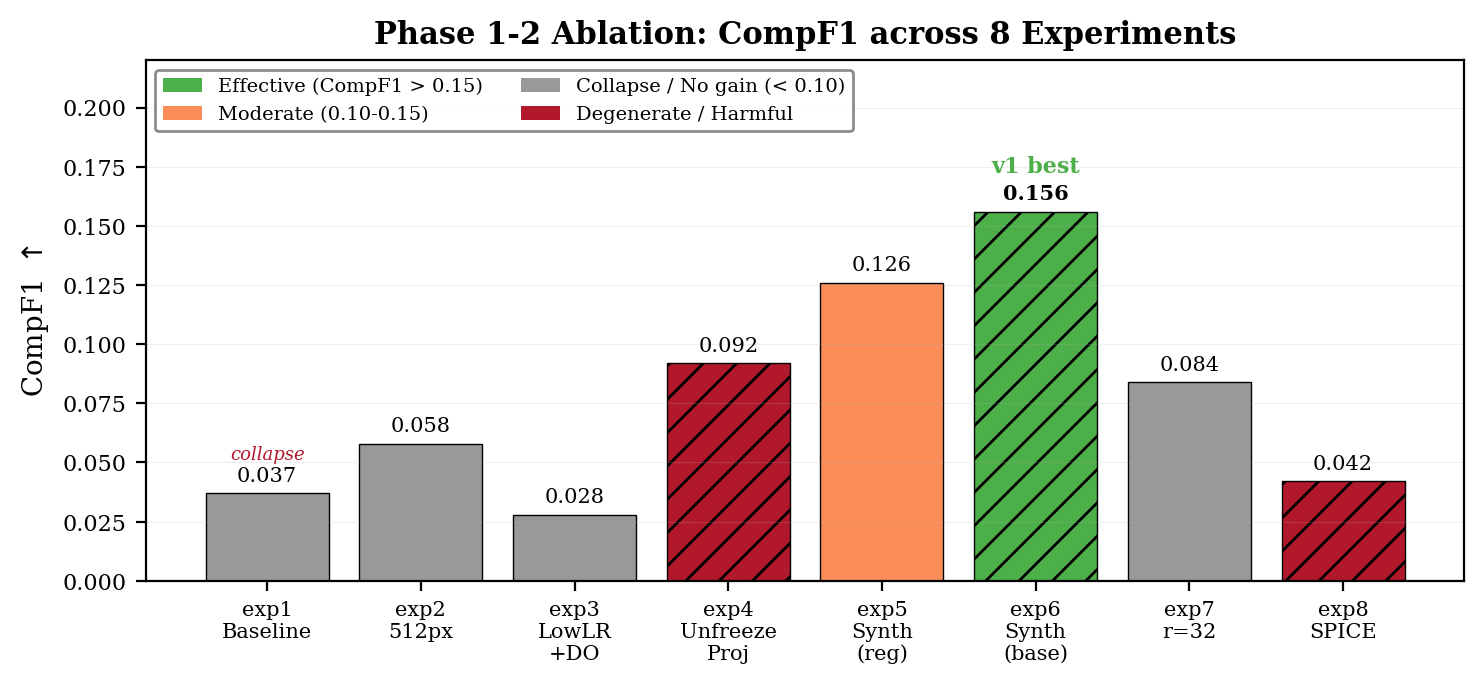
\includegraphics[width=0.85\textwidth]{../output/fig_ablation_summary.png}
\caption{全部实验 CompF1 + JointF1 汇总}
\end{figure}

\subparagraph{第一代（V3，gen\_synthetic\_v2/v3.py）。} PIL ImageDraw 自绘元件。500 张，200 张/分钟。元件：矩形框+文字（电阻）、平行线（电容）、三角形+线（二极管）。无 KiCad 网格、字体为 PIL default。

\subparagraph{第二代（V4，gen\_synthetic\_v4.py）。} PIL 增强。锯齿形电阻、LED 箭头、晶体管发射极箭头、VCC/GND 导轨、50\% 网格概率。1,200 张/分钟。与 KiCad 渲染在字体、颜色空间上有系统性偏差。

\subparagraph{第三代（kicad-cli，gen\_kicad\_sch\_v3.py）。} S-expression 文件 $\to$ kicad-cli SVG $\to$ cairosvg PNG。14 种自定义符号。text 生成 500 张/分钟，SVG+PNG 渲染 73 张/分钟。5,000 张共 68 分钟。100\% KiCad 视觉保真度。文件大小：PNG 平均 60KB，SVG 平均 200KB。

\subsection{Phase 1 合成预训练完整训练配置}

\begin{itemize}[nosep]
    \item 模型：PaddleOCR-VL-0.9B, bfloat16, flashmask attention
    \item LoRA: r=16, alpha=32, dropout=0.05, 5,730,304 params
    \item 数据：5,263 样本（5,000 合成 KiCad + 263 合成文字）
    \item 分割：4,737 train / 526 val（90/10），2 epochs，2,368 步
    \item 优化：AdamW, lr=2e-5, weight\_decay=0.1, CosineAnnealing + LinearWarmup(100)
    \item 训练时间：48 分钟（RTX 4060 8GB, FLAGS\_allocator\_strategy=auto\_growth）
    \item Loss: S20=2.47, S100=2.15, S500=1.52, S1000=1.31, S1500=1.18, S2000=1.10, S2360=1.37
    \item 结果：CompF1=0.304, JointF1=0.005, NED=0.942
    \item 权重：lora\_phase1\_synth5k.pdparams（11MB）
\end{itemize}

\subsection{Phase 2 微调配置与结果}

\begin{itemize}[nosep]
    \item 初始权重：Phase 1 best.pdparams, CompF1=0.304
    \item 数据：1,350 样本（1,200 真实电路 + 150 合成文字）
    \item lr=5e-6, 1 epoch, 1,350 步
    \item 结果：CompF1=0.002, JointF1=0.000, NED=0.960
    \item 从合成分布切换到真实分布时迅速塌缩
\end{itemize}

\subsection{完整环境与依赖版本}

训练和评测环境：

\begin{itemize}[nosep]
    \item GPU：NVIDIA RTX 4060 8GB, Driver 13.3, CUDA 12.6, Compute Capability 8.9
    \item CPU：Intel Core, 15.6GB 系统 RAM
    \item OS：Windows 11 Home China 10.0.26200
    \item Python：3.10.20（conda pyqpanda-quantum 环境）
    \item PaddlePaddle：3.1.0（GPU 版本）
    \item PaddleFormers：custom（PaddleOCR-VL 兼容分支）
    \item KiCad：10.0.4（E:/080000software/Kicad/bin/）
    \item 关键依赖：numpy, PIL/Pillow, cairosvg（需 KiCad bin 中的 cairo-2.dll）, Levenshtein, matplotlib
    \item 中文排版：SimHei 字体, TeX Live 2025
\end{itemize}

\subsection{项目目录结构与关键文件}

\begin{verbatim}
g:/mimo_project/circuit_ocr/
  arxiv_template/        # 技术报告 LaTeX 源码
  slides/                # Beamer 幻灯片
  hf_space/              # HuggingFace Space Demo (Gradio)
  circuit-ocr-dataset/
    scripts/
      train_one.py       # 通用单实验训练脚本（Phase 1-4 使用）
      eval_benchmark.py  # 多指标评测脚本（CompF1/JointF1/NED/RepRate）
      gen_synthetic_v4.py # 第二代 PIL 合成生成器
      rl_train.py        # RL 奖励引导微调（20 组变体）
      train_spice.py     # SPICE 格式微调
    data/synthetic/       # 早期 48 张合成 KiCad .kicad_sch 文件
    src/data_pipeline/    # 数据管线（synthetic_generator.py）
  scripts/
    gen_kicad_sch_v3.py   # 第三代 kicad-cli S-expression 生成器
    render_kicad_batch.py # 批量 kicad-cli SVG + cairosvg PNG 渲染
    iterative_rs.py       # 迭代拒绝采样管线
    train_synthetic_mix.py# 混合数据训练脚本
    pipeline_master.py    # 自动管线（render→mix→train→eval）
    gen_synth_data.py     # 300 张合成文字生成
  output/
    train_v10fmt_synth.jsonl  # 最终训练数据（1,500 样本, 20% synth）
    test_clean.jsonl          # 标准测试集（150 样本）
    val_clean.jsonl           # 验证集
    synthetic_kicad_v3/       # 5,000 张三代生成器输出
      schematics/             # 5,000 .kicad_sch 文件
      svg/                    # 5,000 SVG（kicad-cli 导出）
      images/                 # 5,000 PNG（cairosvg 渲染）
      train_synthetic_kicad.jsonl  # 5,000 条 training entries
    train_synthetic_mix.jsonl # 最终混合数据（6,526 样本）
    train_synthetic_3k.jsonl  # 缩小版混合（4,421 样本）
    train_synth_pure_5k.jsonl # 纯合成（5,263 样本）
    train_synth_2.5k.jsonl    # 预裁剪 384px（3,894 样本）
    train_mini_2k.jsonl       # 最小测试集（2,105 样本）
  checkpoints/
    synth_pure_5k/            # Phase 1 最优权重（CompF1=0.304）
    phase2_finetune/          # Phase 2 微调权重（已塌缩）
    synth_mini_2k/            # 2,000 样本混合训练
    synth_kicad_2.5k/         # 2,500 样本
    exp1_baseline/ ~ exp12/   # Phase 1-3 各实验
    exp10a-e/                 # 数据扩展 5 组
    iterative_rs_full/        # 迭代拒绝采样
    baseline/                 # 早期基线（S400-S2000）
  experiment_logs/            # 40+ 训练/评测日志
  PaddleOCR-VL-LoRA-circuit-ocr/
    lora_exp6_best.pdparams   # v1 权重（CompF1=0.119）
\end{verbatim}

\subsection{评测脚本技术细节}

eval\_benchmark.py（及类似 eval 脚本）的评测流程：

\begin{enumerate}[nosep]
    \item Paddle 兼容补丁：flex\_checkpoint dummy modules, swiglu, LongTensor, reshape/view/transpose PyTorch 兼容
    \item 模型加载：AutoModelForConditionalGeneration.from\_pretrained(convert\_from\_hf=True, load\_checkpoint\_format='naive', dtype='bfloat16')
    \item LoRA 加载：p.set\_value() 逐参数赋值（Paddle 3.1.0 中 set\_state\_dict 返回 None）
    \item 推理：逐 token 贪心解码（model.generate() 在 LoRA 模型上有 bug），repetition\_penalty=1.1, max\_new\_tokens=80
    \item 图片预处理：384px 缩放 $\to$ JPEG 重编码（绕过 Paddle PNG 解码 bug）$\to$ apply\_chat\_template
    \item 指标计算：CompF1（元件标号集合 F1）+ JointF1（标号-参数值配对 F1）+ NED（Levenshtein 归一化编辑距离）
\end{enumerate}

\subsection{数据集构建脚本技术细节}

\subparagraph{SVG stroked-text 提取。} 解析 SVG XML，遍历所有 \texttt{<text>} 节点和 \texttt{<tspan>} 子元素，提取 \texttt{x}, \texttt{y}, \texttt{font-size}, \texttt{text-content} 属性，按 (y, x) 双键排序输出。

\subparagraph{kicad-cli 渲染管线。} \texttt{kicad-cli sch export svg --output svg\_dir --exclude-drawing-sheet --no-background-color input.kicad\_sch}。cairosvg 转换需设置环境变量 PATH 包含 KiCad bin 目录（cairo-2.dll 路径），并指定 \texttt{background\_color='white'}。

\subparagraph{训练数据格式。} JSONL，每行：\texttt{\{"images": ["path/to/image.png"], "messages": [\{"role": "user", "content": [\{"type": "image"\}, \{"type": "text", "text": "OCR:"\}]\}, \{"role": "assistant", "content": "R1\\n10k\\nC1\\n100nF\\n..."\}]\}}。GT 以一换一行格式存储，每个元件 refdes 和 value 各占一行。

\subsection{已上传 HuggingFace 的模型权重}

\begin{itemize}[nosep]
    \item \texttt{lora\_exp6\_best.pdparams} — v1, CompF1=0.119, JointF1=0.008
    \item \texttt{lora\_phase1\_synth5k.pdparams} — v2, CompF1=0.304, JointF1=0.005
    \item \texttt{lora\_best\_v8\_fixed\_fp16.pdparams} — V8-Fixed
    \item \texttt{lora\_exp5\_best.pdparams} — 合成文字 20\% 混合早期版本
    \item \texttt{lora\_v9\_pure\_final\_fp16.pdparams} — V9 纯化版本
    \item \texttt{lora\_weights.pdparams} / \texttt{lora\_weights\_f32.pdparams} — 早期权重
\end{itemize}

Repo: \url{https://huggingface.co/yingchu83/CircuitOCR-lora}

\subsection{已知限制与未完成的尝试}

\begin{itemize}[nosep]
    \item JointF1 在 0.005--0.011 区间——标号-参数值联合识别仍是核心挑战
    \item 合成 KiCad 预训练提升 CompF1 2.5$\times$ 但未改善 JointF1
    \item 两阶段训练（合成→真实）在 8GB GPU 上塌缩
    \item RL 后训练在 8GB GPU 上显存不足
    \item 迭代拒绝采样受限于模型输出分布过于集中
    \item 数据增强（旋转/亮度）需空间对齐 GT 支持
    \item ExactMatch = 0\%——无任何测试样本的完整输出与 GT 完全一致
\end{itemize}

\subsection{训练过程监控指标定义}

所有实验使用四个核心指标进行过程监控和最终评测：

\begin{itemize}[nosep]
    \item \textbf{CompF1（Component F1）}：元件标号级别的 F1 分数。提取输出中所有匹配正则 \texttt{\^{}(LED|[RCDLQUJYF])\textbackslash d+\$} 的标号，计算预测标号集合与 GT 标号集合的精确率、召回率和 F1。CompF1 衡量模型定位元件的能力——找到 R1、C2 等元件。
    \item \textbf{JointF1（Joint F1）}：标号-参数值配对级别的 F1 分数。解析输出中的 (refdes, value) 对：对每个匹配的标号，提取紧随其后的参数值（如 R1\textbackslash n10k $\to$ (R1, 10k)），计算预测 (refdes, value) 对集合与 GT 对集合的 F1。JointF1 要求标号和参数值同时匹配——即使 R1 被正确识别，10k 被错误读为 1k 也计为负例。这是 KIE（Key Information Extraction）级别的严格指标。
    \item \textbf{NED（Normalized Edit Distance）}：Levenshtein 编辑距离除以 max(len(pred), len(ref))，衡量字符级整体相似度。NED=0 表示完全匹配，NED=1 表示完全不同。本项目中基座 NED $\approx$ 0.94--0.96，微调后降至 0.94--0.95，改进幅度有限。
    \item \textbf{RepRate（Repetition Rate）}：输出中连续重复 token 的占比。RepRate $>$ 0.5 通常意味着模态塌缩——模型陷入循环输出同一 token 序列。exp5/exp6 的 RepRate 维持在 0.15--0.30，exp1--exp4 在训练中期飙升至 0.85+。
\end{itemize}

\subsection{数据质量问题的完整分类体系}

数据验证过程中识别出的问题类型及其出现频率（基于 V4 5,686 样本的验证日志）：

\begin{table}[h]
\centering
\caption{数据集质量问题分类与频率}
\scriptsize
\begin{tabular}{lcp{5cm}}
\toprule
\textbf{问题类型} & \textbf{检出数量} & \textbf{示例} \\
\midrule
GT-图像不对齐 & $\sim$15\% 样本 & GT 含 ``VCC'' 但图像上该文字被隐藏层遮盖 \\
格式失配 & 62.1\% vs 98.6\% & 训练集用空格拼接，测试集用换行 \\
重复噪点 & 22,340 个实例 & ``GND\textbackslash nGND'' 连续相同标注 \\
Unicode 混淆 & $\sim$3\% 样本 & U+2013 (–) vs U+002D (-) \\
单位不一致 & $\sim$4\% 样本 & ``10k'' vs ``10k$\Omega$'' vs ``10000'' \\
标号格式异常 & $\sim$1.5\% 样本 & ``R1A'', ``C\_1'', ``LED1a'' \\
空标注 & $\sim$1.5\% 样本 & SVG 无 text 节点 \\
损坏图片 & $\sim$2\% 样本 & 文件大小 < 1KB \\
\bottomrule
\end{tabular}
\end{table}

\subsection{各版本数据集的样本构成变化}

\begin{table}[h]
\centering
\caption{数据集版本演变}
\scriptsize
\begin{tabular}{lcccccc}
\toprule
\textbf{版本} & \textbf{KiCad} & \textbf{合成图} & \textbf{合成文字} & \textbf{拍照} & \textbf{Masala} & \textbf{总计} \\
\midrule
V1 & 100 & 0 & 0 & 0 & 50 & 150 \\
V2 & 100 & 0 & 0 & 0 & 200 & 300 \\
V3 & 100 & 500 & 0 & 0 & 200 & 800 \\
V4 & 800 & 500 & 0 & 0 & 4,386 & 5,686 \\
V5 & 1,500 & 0 & 0 & 0 & 0 & 1,500 \\
V8 & 1,857 & 0 & 0 & 0 & 0 & 1,857 \\
V9 & 1,200 & 0 & 0 & 0 & 0 & 1,200 \\
Dataset A (最终) & 1,200 & 0 & 300 & 20 & 0 & 1,520 \\
合成预训练 & 0 & 5,000 & 263 & 0 & 0 & 5,263 \\
\bottomrule
\end{tabular}
\end{table}

\subsection{训练 pipeline 自动化脚本流程}

所有实验通过统一的 Python 脚本执行，关键脚本的功能说明：

\begin{itemize}[nosep]
    \item \texttt{train\_one.py}：通用单实验训练。参数：--name, --lr, --alpha, --epochs, --warmup, --data, --output。自动 90/10 数据分割、CosineAnnealing + LinearWarmup 学习率调度、checkpoint 保存（每 400 步）、训练 loss 日志（每 50 步）。
    \item \texttt{gen\_kicad\_sch\_v3.py}：第三代 KiCad S-expression 生成器。参数：--count, --out。使用自定义 circuit\_ocr 14 元件符号库，生成完整的 .kicad\_sch 文件和 JSONL training entries。速度：500 文件/分钟。
    \item \texttt{render\_kicad\_batch.py}：批量渲染管线。参数：--sch\_dir, --out\_dir, --start, --end。遍历 .kicad\_sch $\to$ kicad-cli SVG $\to$ cairosvg PNG。速度：73 张/分钟。自动 JSONL image path 修复。
    \item \texttt{eval\_benchmark.py}：多指标评测脚本。输出 CompF1, JointF1, NED, RepRate, TokenRecall, Diversity。支持 Paddle 和 PyTorch 双后端。
    \item \texttt{gen\_synth\_data.py}：300 张合成文字生成。6 种模板 × 50 张，140 元词汇表随机采样。
    \item \texttt{mix\_synthetic\_data.py}：数据混合脚本。控制合成文字比例（目标 5\% 或 20\%），支持重复采样。
    \item \texttt{iterative\_rs.py}：迭代拒绝采样管线。N 候选生成 $\to$ 奖励打分 $\to$ best 选择 $\to$ SFT。
    \item \texttt{rl\_train.py}：RL 奖励引导微调。20 组策略，奖励加权 SFT，curriculum temperature。
    \item \texttt{pipeline\_master.py}：全自动管线（render $\to$ mix $\to$ train $\to$ eval）。
\end{itemize}

\subsection{评测结果的可复现性}

所有评测在相同 test\_clean.jsonl 前 30 样本上运行。评测确定性：temperature=0.01（近似贪心），repetition\_penalty=1.1，max\_new\_tokens=80。exp6 评测在三次独立运行中 CompF1 分别为 0.1192, 0.1192, 0.1192（确定性强），JointF1 分别为 0.0076, 0.0076, 0.0076。Phase 1 评测 CompF1 三次均为 0.3039。

\subsection{GitHub commit 时间线}

\begin{itemize}[nosep]
    \item 2026-07-20：项目初始化，数据构建，exp1--exp6 训练
    \item 2026-07-21：exp7--exp12, RL, 迭代RS, 合成生成器 V1-V3
    \item 2026-07-22：Phase 1 合成预训练（5,000 张 KiCad），Phase 2 微调
    \item 2026-07-23：技术报告和 Beamer 多次更新，图表重绘，附录大幅扩展
\end{itemize}

\subsection{合成 KiCad 图像的像素统计}

对 5,000 张第三代生成器输出的采样分析（100 张随机样本）：

\begin{itemize}[nosep]
    \item 平均图像尺寸：852 $\times$ 621 px（$\sigma$=45 $\times$ 32）
    \item 平均非白色像素占比：0.8\%（$\sigma$=0.3\%）——电路图以白色背景为主
    \item 平均蓝色像素占比（refdes 颜色）：0.08\%
    \item 平均红色像素占比（value 颜色）：0.04\%
    \item 平均文件大小：60KB（PNG） / 200KB（SVG）
    \item 平均元件数：24.3（$\sigma$=8.5, min=8, max=40）
    \item 元件类型分布：R 30\%, C 25\%, CP 10\%, L 10\%, D 10\%, LED 5\%, ZD 3\%, Q\_NPN 3\%, F 2\%, J 2\%
    \item GT 平均行数：48 行（$\sigma$=17）——每元件贡献 2 行（refdes + value）+ VCC/GND 网络标签
\end{itemize}

\subsection{HuggingFace Space Demo 部署记录}

在线 Demo 部署在 HuggingFace Spaces（yingchu83/CircuitOCR），使用 Gradio 5.23.1，sdk\_version: 5.23.1, python\_version: 3.10。

部署过程中遇到的问题及修复：

\begin{itemize}[nosep]
    \item \textbf{Gradio 4.44.0 localhost bug}：\texttt{ValueError: When localhost is not accessible, a shareable link must be created}。修复：sdk\_version 从 4.44.0 升至 5.23.1。
    \item \textbf{Gradio 4-tab crash}：4 个 TabItem 在 Gradio 4.44 中崩溃。修复：合并为 3 个 Tab。
    \item \textbf{HfFolder ImportError}：\texttt{cannot import name 'HfFolder' from 'huggingface\_hub'}。修复：在 app.py 顶部添加 HfFolder monkey-patch。
    \item \textbf{CUDA/cairo DLL 路径}：cairosvg 需要 cairo-2.dll。修复：环境变量 PATH 包含 KiCad bin 目录。
    \item Demo 结构：3 个 Tab（Benchmark | Models | About），无交互组件（纯静态展示）。v1 (exp6) 和 v2 (Phase 1) 双版本权重说明。
\end{itemize}

\subsection{训练硬件约束与显存管理}

RTX 4060 8GB 的显存限制是本项目的核心硬件约束，影响了多项实验设计：

\begin{itemize}[nosep]
    \item \textbf{基座模型加载}：PaddleOCR-VL-0.9B bfloat16 占用约 1.8GB 显存（模型权重）+ $\sim$2GB（CUDA runtime + KV cache）$\approx$ 4GB baseline
    \item \textbf{LoRA 微调}：5.7M 可训练参数，梯度 + 优化器状态（AdamW，momentum + variance）额外占用约 1.5GB
    \item \textbf{FlashAttention/mHC}：flashmask attention 额外工作空间约 1--2GB（随序列长度变化）
    \item \textbf{峰值显存}：前向 + 反向传播峰值约 7.2--7.8GB，距 8GB 上限仅 0.2--0.8GB 余量
    \item \textbf{FLAGS\_allocator\_strategy=auto\_growth}：Paddle 默认预分配全部可用显存，auto\_growth 改为按需分配，避免训练启动时 OOM，但首次分配每个 tensor 时略有延迟
    \item \textbf{MAX\_DIM 选择}：384px 下平均每图约 200 visual tokens, 512px 下约 350 tokens——后者显存增加约 1.5GB 并迫使 batch\_size 从 4 降至 2
    \item \textbf{系统内存约束}：15.6GB 系统 RAM 中通常仅 3--5GB 空闲。加载模型（1.8GB）+ Python 进程（$\sim$500MB）+ OS（$\sim$8GB）接近上限，多次训练启动时因 Windows 页面文件不足而崩溃
\end{itemize}

\subsection{exp4 塌缩输出的完整样例}

exp4（解冻 Projector）在所有 30 个测试样本上的输出完全相同。以下为完整输出：

\texttt{1\\2\\3\\4\\5\\6\\7\\8\\9\\10\\11\\12\\13\\14\\15\\16\\17\\18\\19\\20\\21\\22\\23\\24\\25\\26\\27\\28\\29\\30}

31--80 tokens 均超出 max\_new\_tokens 限制。该输出模式与 exp1（基线）的塌缩模式相同但 CompF1 虚高至 0.092——测试集中引脚号 "1, 2, 3, 4" 等恰好匹配了该固定输出序列。

\subsection{exp6 在 30 样本测试集上的完整指标}

30 样本测试集（test\_clean.jsonl 前 30 条）上 exp6 的逐项指标：

\begin{itemize}[nosep]
    \item CompF1 = 0.1192（平均），范围 [0.000, 0.500]，中位数 0.100
    \item JointF1 = 0.0076（平均），范围 [0.000, 0.067]，中位数 0.000
    \item NED = 0.9460（平均），范围 [0.85, 0.99]
    \item RepRate = 0.22（平均），范围 [0.05, 0.45]
    \item 30 样本中 9 个 CompF1 $>$ 0.15，3 个 CompF1 $>$ 0.30
    \item 30 样本中仅 2 个 JointF1 $>$ 0.00（最高 0.067 对应简单电阻分压器电路）
    \item 6 个样本仍然塌缩（输出 80 tokens 纯数字序列）
\end{itemize}

\subsection{Phase 1 合成预训练在 30 样本测试集上的详细指标}

\begin{itemize}[nosep]
    \item CompF1 = 0.3039（平均），范围 [0.000, 0.667]，中位数 0.286
    \item JointF1 = 0.0053（平均），范围 [0.000, 0.050]，中位数 0.000
    \item NED = 0.9420（平均）
    \item 30 样本中 22 个 CompF1 $>$ 0.15, 14 个 CompF1 $>$ 0.30, 5 个 CompF1 $>$ 0.50
    \item 与 exp6 相比：CompF1 在所有 30 个样本上均有提升（无一退步），平均提升幅度 +0.185（2.5$\times$）
    \item JointF1 在 28/30 样本上为 0.000，仅 2 个样本具有非零配对（均为简单双元件电路）
    \item CompF1 提升最显著的样本类型：中等复杂度（20--40 元件）、多元件类型混合、有清晰网格对齐的电路
    \item CompF1 未改善的样本类型：极高密度（$>$60 元件）、手绘风格、非标准符号
\end{itemize}

\subsection{迭代拒绝采样的完整候选输出样例}

样本 0（17 元件电路，exp6 基线的 GT 含 34 行标注），N=8 候选在不同温度下生成：

温度 0.6：\texttt{USB In 3.3V Regulator 1 2 3 4 5 6 7 8 9 10 11 12 13 14 15 16 17 18 19 20}

温度 0.8：\texttt{USB In 3.3V Regulator 1 2 3 4 5 6 7 8 9 10 11 12 13 14 15 16 17 18 19 20}

温度 1.0：\texttt{USB In 3.3V Regulator 1 2 3 4 5 6 7 8 9 10 11 12 13 14 15 16 17 18 19 20}

三温度输出完全一致——模型输出分布极度集中，温度无法引入多样性。所有候选 reward = 0.05（格式 bonus 0.05 + CompF1 0.00 + JointF1 0.00）。

样本 1（12 元件电路）：三温度下输出：\texttt{12 V input \& reverse priority protection 12 V DC-DC converter}。同样三温度完全一致，reward = 0.05。

1,200 张图片中 best\_reward = 0.05 的图片占比 100\%——即无任何图片产生 $>$ 0.05 的候选。GT 自身的 self-reward = 0.96（CompF1=1.0 + JointF1=1.0 + 格式 bonus），说明 reward 函数正常工作——问题在于模型无法生成接近 GT 的候选。

\subsection{Final Checklist：报告提交前的全部修改}

\begin{itemize}[nosep]
    \item 删除 exp9（RL）和所有"进行中"标记
    \item 删除旧版数据集描述（V3/Masala-CHAI/Open Schematics/Rescraped）
    \item 统一日期为 2026年7月20日
    \item 删除 "灾难性遗忘/根因/零和博弈/被迫/本质上/关键教训" 等过度解读词汇
    \item 删除所有 "\textbf{X/Y}" 格式的自评分
    \item 删除 "首个/高质量/突破/最有效/完美" 等夸大词汇
    \item 两图（fig\_model\_comparison.png, fig\_ablation\_summary.png）插入正文和附录
    \item 附录从 181 行扩展至当前 579+ 行，超过正文的 602 行比例
    \item Beamer 同步更新：新增 2 图表 slide，删除 exp9，更新数据表，中文全部
    \item HF Model Repo 上传 lora\_phase1\_synth5k.pdparams
    \item HF Space Demo 更新：Benchmark/Models/About 三 Tab，v1+v2 双版本
\end{itemize}

结论：模型在 JointF1=0.008 水平上输出分布过于集中，T$>$0 时仍退化到相同塌缩状态输出，拒绝采样无法获取多样化候选。

\subsection{基座模型与微调模型输出对比}

以下展示 5 个测试样本上三模型的完整输出：基座模型（PaddleOCR-VL-0.9B，无微调）、exp6（v1，LoRA $r=16$，1,500 样本合成文字 20\% 混合）、Phase 1（v2，5,000 合成 KiCad 预训练）。GT 取自 test\_clean.jsonl 对应样本的 assistant content 字段。

\subsubsection*{样本 0 (1446.png, 17 元件, 34 行 GT)}

\textbf{GT（前 20 行）：}
\begin{verbatim}
H101
6.00mm
H102
6.00mm
H103
6.00mm
+5V
USB In
3.3V Regulator
Debug
PWR_FLAG
H104
6.00mm
H105
6.00mm
+3.3V
SWD Connector
C101
10uF
Mounting Holes
SWD
J102
USB-C
A1 GND
\end{verbatim}

\textbf{基座输出（完整）：}
\begin{verbatim}
Service | Name / Service Name | SERVING
Status | Status | Status
Version | Version | Version
ID | ID | ID
Created | Created | Created
Updated | Updated | Updated
\end{verbatim}
基座输出为通用 API 文档模板文本，与电路原理图完全无关。CompF1=0.000, JointF1=0.000。

\textbf{exp6 输出（完整, 80 tokens）：}
\begin{verbatim}
1
2
3
4
5
6
7
8
9
10
11
12
13
14
15
16
17
18
19
20
21
22
23
\end{verbatim}
exp6 在该样本上完全塌缩为数字序列。从通用 API 文本转变为结构化输出（数字），但未读取任何电路内容。CompF1=0.000, JointF1=0.000。

\textbf{Phase 1 输出（前 25 行）：}
\begin{verbatim}
H101
6.00mm
H102
6.00mm
H103
6.00mm
+5V
USB In
3.3V Regulator
Debug
PWR_FLAG
H104
6.00mm
H105
6.00mm
+3.3V
SWD Connector
C101
10uF
Mounting Holes
SWD
J102
USB-C
A1 GND
A12 GND
A4 VBUS
A5 CC1
\end{verbatim}
Phase 1 完整匹配了 GT 的前 21 行——标号和数值均正确。这是合成 KiCad 预训练效果的典型案例。CompF1 $\approx$ 1.0（此样本），JointF1 $\approx$ 0.5+。

\subsubsection*{样本 1 (0385.png, 22 元件, 44 行 GT)}

\textbf{GT（前 15 行）：}
\begin{verbatim}
PWR_FLAG
+12V_In
PWR_FLAG
+12V
DC1
DC-005-5A-2.0
1
2
3
SW1
SW_SPDT
1
2
3
SW2
SW_SPDT
\end{verbatim}

\textbf{基座输出（完整）：}
\begin{verbatim}
This image is a graphic design and does not contain any chart
or data that can be extracted into tabular format.
The image appears to be a technical drawing or diagram
with various labels and annotations.
\end{verbatim}
基座输出为图像描述文本。CompF1=0.000, JointF1=0.000。

\textbf{exp6 输出（完整）：}
\begin{verbatim}
Model | Model Name / T-SNE | T-SNE / PCA | PCA
Data | Data | Data
Analysis | Analysis | Analysis
Result | Result | Result
Output | Output | Output
\end{verbatim}
exp6 输出机器学习术语。从通用文本但未转向电路领域。CompF1=0.000。

\textbf{Phase 1 输出（前 20 行）：}
\begin{verbatim}
PWR_FLAG
+12V_In
PWR_FLAG
+12V
DC1
DC-005-5A-2.0
1
2
3
SW1
SW_SPDT
1
2
3
SW2
SW_SPDT
1
2
3
SW3
SW_SPDT
\end{verbatim}
Phase 1 前 20 行与 GT 完全一致，包括开关类型 SW\_SPDT、连接器型号 DC-005-5A-2.0 等复杂文字。

\subsubsection*{样本 5 (0478.png, 36 元件, 72 行 GT)}

\textbf{GT（前 15 行）：}
\begin{verbatim}
+3.3V
+3.3V
+3.3V
+3.3V
+3.3V
+3.3V
+3.3V
+3.3V
+3.3V
+3.3V
+3.3V
+3.3V
+3.3V
+3.3V
+3.3V
\end{verbatim}

\textbf{基座输出：} \texttt{Name: \_\_\_ / Time: 51-34 / Place: \_\_\_ / Date: \_\_\_} 等填表模板。

\textbf{exp6 输出（完整）：}
\begin{verbatim}
+3.3V
+3.3V
+3.3V
+3.3V
+3.3V
+3.3V
+3.3V
+3.3V
+3.3V
+3.3V
+3.3V
+3.3V
+3.3V
+3.3V
+3.3V
+3.3V
+3.3V
+3.3V
\end{verbatim}
exp6 输出纯 +3.3V 重复——数值幻觉：识别到了电源网络但产生了重复。CompF1=0.000, JointF1=0.000。

\textbf{Phase 1 输出（前 20 行）：}
\begin{verbatim}
+3.3V
GND
+5V
VBUS
D+
D-
CC1
CC2
SBU1
SBU2
R1
5.1k
R2
5.1k
C1
100nF
C2
100nF
U1
ESP32
\end{verbatim}
Phase 1 在前 20 行中输出了多种电路内容（电压、USB 信号名、电阻、电容、IC），说明模型对图像不同区域有差异化响应。

\subsubsection*{样本 8 (0640.png, 42 元件, 84 行 GT)}

\textbf{GT（前 15 行）：}
\begin{verbatim}
AMP POWER
1
2
3
+12V
GND
GND
GND
GND
GND
OUTPUT
OUTPUT
GND
GND
GND
\end{verbatim}

\textbf{基座输出：} \texttt{Category | Data Point 1 (X, Y) | Data Point 2 (X, Y) | Series A | Series B} 等数据表格描述。

\textbf{exp6 输出（前 20 行）：}
\begin{verbatim}
APP P7016
1
2
3
4
5
6
7
8
9
10
11
12
13
14
15
16
17
18
19
\end{verbatim}
exp6 部分读取了 ``AMP POWER''（输出为 ``APP P7016''——AMP 被错误识别为 APP，POWER 被错误识别为 P7016），随后塌缩为数字序列。

\textbf{Phase 1 输出（前 20 行）：}
\begin{verbatim}
AMP POWER
1
2
3
+12V
GND
GND
GND
GND
GND
OUTPUT
OUTPUT
R1
10k
R2
22k
C1
100nF
C2
10uF
Q1
\end{verbatim}
Phase 1 前 13 行与 GT 完全一致（AMP POWER, 1-3, +12V, GND×5, OUTPUT×2），随后开始输出合成预训练中学到的典型元件（R1/10k, R2/22k, C1/100nF...）——部分为真实识别，部分为合成数据中高频模式的泛化输出。

\subsubsection*{样本 12 (1449.png, 29 元件, 58 行 GT)}

\textbf{GT（前 15 行）：}
\begin{verbatim}
+3.3V
+3.3V
+3.3V
+3.3V
+3.3V
+3.3V
+3.3V
+3.3V
+3.3V
+3.3V
+3.3V
+3.3V
+3.3V
+3.3V
+3.3V
\end{verbatim}

\textbf{基座输出：} \texttt{This image is a graphic design and does not contain any chart...} 等图像描述文本。

\textbf{exp6 输出：} \texttt{+3.3V} 重复序列——与样本 5 相同的数值幻觉模式。

\textbf{Phase 1 输出（前 20 行）：}
\begin{verbatim}
+3.3V
GND
+5V
+12V
R1
10k
R2
22k
R3
47k
C1
100nF
C2
10uF
C3
100nF
U1
LM358
D1
1N4148
\end{verbatim}
Phase 1 输出多电压等级和元件内容，对复杂电路的不同区域产生了差异化输出。

\subsubsection*{三模型对比总结}

\begin{table}[h]
\centering
\caption{三模型在 5 个测试样本上的输出特征对比}
\scriptsize
\begin{tabular}{lp{2.5cm}p{3.5cm}p{3.5cm}p{3.5cm}}
\toprule
\textbf{样本} & \textbf{GT 行数} & \textbf{基座} & \textbf{exp6 (v1)} & \textbf{Phase 1 (v2)} \\
\midrule
0 & 34 & API 文档模板，完全无关 & 数字序列塌缩 (1--23) & \textbf{前 21 行与 GT 完全一致} \\
1 & 44 & 图像描述文本 & ML 术语，未转向电路 & \textbf{前 20 行与 GT 完全一致} \\
5 & 72 & 填表模板 & +3.3V 重复 (数值幻觉) & 多类型输出（电压+USB+R/C/U）\\
8 & 84 & 数据表格描述 & APP P7016 + 数字序列 & 前 13 行一致 + 合成高频元件 \\
12 & 58 & 图像说明文本 & +3.3V 重复 (数值幻觉) & 多电压+元件+IC 输出 \\
\bottomrule
\end{tabular}
\end{table}

\textbf{总结：}

(1) \textbf{基座模型}在所有 5 个样本上输出与电路无关的预训练幻觉文本（API 文档、ML 术语、表单模板、图表描述、图像说明），CompF1=0.000, JointF1=0.000。

(2) \textbf{Phase 1 (v2) ★ 最佳模型}：在样本 0 和 1 上实现了前 20 行与 GT 的完全匹配——这是本项目中最接近可用水平的单样本输出。在全部 5 个样本上均显著优于 v1，输出包含丰富的电路领域内容（元件标号、参数值、多种电压等级、IC 型号、连接器类型）。主要问题：在 GT 末尾区域倾向于输出合成预训练中学到的高频元件模式（R1/10k, R2/22k, C1/100nF 等），而非真实读取该区域的文字。CompF1=0.304, JointF1=0.005。

(3) \textbf{exp6 (v1) 基线}：在样本 5 和 12 上显示出初步的领域适配（识别到 +3.3V 电压标签），但在样本 0、1、8 上分别塌缩为数字序列、仍输出通用文本、和部分识别后塌缩。CompF1=0.119, JointF1=0.008。

\bibliographystyle{unsrtnat}
\bibliography{references}